\section{Evaluation}
\label{section:evaluation}
In the following chapter the mobile implication of \gls{see} will be evaluated in a user study.
Therefore, the mobile application will be compared with the desktop version.

This chapter will start with a description of the desktop version and its main differences in section \ref{desktop}.
Continuing with a defined aim and precise hypotheses for the user study in section \ref{aim}.
After sketching the first experiment set up in section \ref{experiment} the actual experiment set up will be discussed in detail in section \ref{real} including the used survey tool, questionnaires and the pilot study.
This chapter will then be closed by discussing the results of the user study in section \ref{results} and talking about the threads of validity in section \ref{sec:validity}.
\subsection{SEE Desktop}
\label{desktop}
In this section the desktop version of \gls{see} will be explained.
In this evaluation the mobile version of \gls{see} will be compared with the desktop version.
Therefore, it is necessary to take a deeper look at the differences between those two versions.
Especially at how the interactions differ and what impact it could have on the user experience.

One outstanding difference from the desktop version to the mobile version is the selection of the interaction modes.
While in the mobile version the menu for the interaction modes is always visible in the desktop version by pressing space a menu screen opens as seen in figure \ref{fig:menu}.
Alternatively interaction modes can be changed by pressing one of the "1-9" keys, which, however requires the user to memorize which number belongs to which mode.

\begin{figure}[htb]
  \centering
  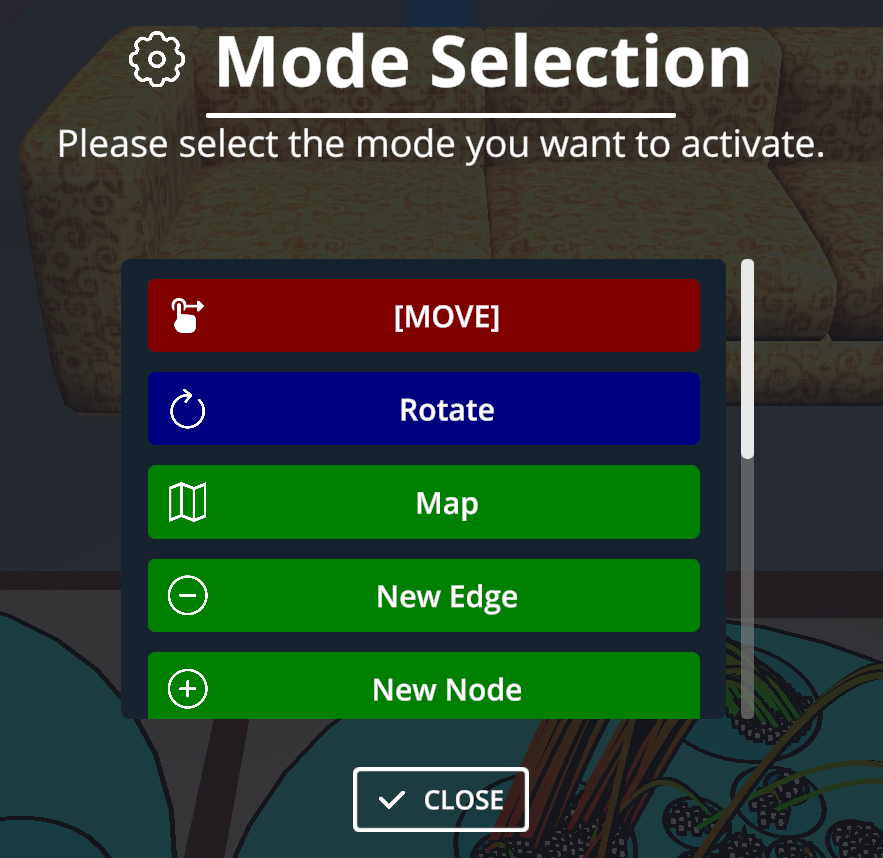
\includegraphics[width=0.8\textwidth]{Evaluation/img/menu.png}
  \caption{The desktop menu for selecting interaction modes.}\label{fig:menu}
\end{figure}

Another difference is the type of user input.
The desktop version uses mouse hovering to display the name of a hovered \gls{node} or \gls{plane}.
This is a faster method then touching the object first in the mobile version.
In addition to that in the mobile version the object also has to be deselected otherwise there will be a lot of \gls{node} and \gls{plane} names displayed, and it will soon get quite messy.
Also, the precision of object selection differs because touch input can never be as precise as selecting with a mouse cursor.
This could force the mobile user to zoom further in because with a touch input it will not be possible to select small objects like it might be with a cursor.
Which, of course, would require more time.

One more key difference is the available keyboard for desktop users.
It allows using \glspl{shortcut}, which makes some menu items unnecessary but also requires the user to memorize those \glspl{shortcut}.
The desktop version for example uses the "R" key in the move and rotation mode to recenter or rerotate a \gls{city}.
In the mobile version on the other side the user will find a button for both actions.
With the right amount of training both actions should probably equal in the amount of time they need but the mobile version sacrifices screen space for those buttons.
If however the user has to type more text like in renaming objects, the common desktop keyboard should come in handy as a study from \cite{kim2014differences} shows that even at a same keyboard size, a virtual one will lack in productivity.
\subsection{Aim and hypothesis}
\label{aim}
The aim of this user study is to answer the research question discussed in section \ref{research}.
In order of answering the research question the finished prototype of the mobile extension shall be evaluated.
Therefore, the system shall be compared on \gls{android} smartphones as well as desktop computers.
Comparing these two use cases shall give insight on how much impact the constraints of mobile devices have on the usability and overall user experience.
To measure the difference between the desktop and the mobile version the following hypotheses will be used.
The two aspects performance and usability will be measured in the following study and each aspect will have a null hypothesis and an alternative hypothesis.
\begin{enumerate}[{label=\alph*)}]
  \item \textbf{Performance:} The time required for a task in \gls{see} desktop will be called $t_D$ and for mobile $t_M$.
        \begin{itemize}
          \item \textit{Null Hypothesis} $H_{a0}$: The time required in \gls{see} desktop is higher or the same as the time required in \gls{see} mobile: $t_D \geq t_M$
          \item \textit{Alternative Hypothesis} $H_{a1}$: The time required in {\gls{see}} desktop is lower as the time required in \gls{see} mobile: $t_D < t_M$
        \end{itemize}
  \item \textbf{Usability:} Two aspects are measured for \gls{usability}. First the \gls{ASQ}-Score as a \gls{post-task} result and second the \gls{sus}-Score as a \gls{post-study} result.
        \begin{enumerate}[label=\roman*)]
          \item \textbf{ASQ:} Once again the aspect has to be split into three child aspects, because the three questions of the \gls{ASQ} are independent:
                \begin{enumerate}[{label=\arabic*)}]
                  \item The \gls{ASQ}-Score for \textit{complexity} for \gls{see} desktop is called $A_{cD}$ and for \gls{see} mobile is called $A_{cM}$
                        \begin{itemize}
                          \item \textit{Null Hypothesis} $H_{b0}$: The \gls{ASQ}-Score for \textit{complexity} is higher or even for \gls{see} mobile than on \gls{see} desktop: $A_{cM} \geq A_{cD}$
                          \item \textit{Alternative Hypothesis} $H_{b1}$: The \gls{ASQ}-Score for \textit{complexity} is higher for \gls{see} desktop than on \gls{see} mobile: $A_{cD} > A_{cM}$
                        \end{itemize}
                  \item The \gls{ASQ}-Score for \textit{effort} for \gls{see} desktop is called $A_{eD}$ and for \gls{see} mobile is called $A_{eM}$
                        \begin{itemize}
                          \item \textit{Null Hypothesis} $H_{b0}$: The \gls{ASQ}-Score for \textit{effort} is higher or even for \gls{see} mobile than on \gls{see} desktop: $A_{eM} \geq A_{eD}$
                          \item \textit{Alternative Hypothesis} $H_{b1}$: The \gls{ASQ}-Score for \textit{effort} is higher for \gls{see} desktop than on \gls{see} mobile: $A_{eD} > A_{eM}$
                        \end{itemize}
                  \item The \gls{ASQ}-Score for \textit{information} for \gls{see} desktop is called $A_{iD}$ and for \gls{see} mobile is called $A_{iM}$
                        \begin{itemize}
                          \item \textit{Null Hypothesis} $H_{b0}$: The \gls{ASQ}-Score for \textit{information} is higher or even for \gls{see} mobile than on \gls{see} desktop: $A_{iM} \geq A_{iD}$
                          \item \textit{Alternative Hypothesis} $H_{b1}$: The \gls{ASQ}-Score for \textit{information} is higher for \gls{see} desktop than on \gls{see} mobile: $A_{iD} > A_{iM}$
                        \end{itemize}
                \end{enumerate}

          \item \textbf{SUS:} The \gls{sus}-Score is called $S_D$ for \gls{see} desktop and $S_M$ for \gls{see} mobile.
                \begin{itemize}
                  \item \textit{Null Hypothesis} $H_{e0}$: The \gls{sus}-Score is higher or even for \gls{see} mobile than for \gls{see} desktop: $S_M \geq S_D$
                  \item \textit{Alternative Hypothesis} $H_{e1}$: The \gls{sus}-Score is lower for \gls{see} mobile than for \gls{see} desktop: $S_M > S_D$
                \end{itemize}
        \end{enumerate}
\end{enumerate}

The experiment will be participated different groups:
\begin{enumerate}
  \item \textbf{\gls{see}-developer:} They are already experienced with \gls{see}-desktop.
        They are also experienced with software development and with first person games because they tried at least \gls{see} itself, which counts as first person game experience.
  \item \textbf{Non-\gls{see}-developer:} This group has to be divided into four subgroups as follows:
        \begin{itemize}
          \item \textbf{Software development and third person game experience:} They are more likely to understand the \gls{city} metaphor and are also more likely to be comfortable with the controls in \gls{see}.
          \item \textbf{Software development experience:} They are more likely to understand the \gls{city} metaphor and therefore might be able to find \glspl{node} faster.
          \item \textbf{First person game experience:} They are also more likely to be comfortable with the controls in \gls{see}.
          \item \textbf{No experience:} They do not benefit from experience and therefore have to learn the most to interact in \gls{see}
        \end{itemize}
\end{enumerate}

After the experiment the two versions of \gls{see} can be compared as well as all above listed groups. 
This should give a detailed answer to the research question of this thesis.
\subsection{Experiment set up}
\label{experiment}
The system shall be tested in two groups each starting with a different device.
Each group does the test on both devices, but one group will start with the mobile application and the other one with the desktop application.
The participants will be assigned random to the groups.
The testers will have various tasks to test the usability of the two applications.
Afterwards the users will get a survey in English to document their impressions.
\begin{figure}[H]
  \centering
  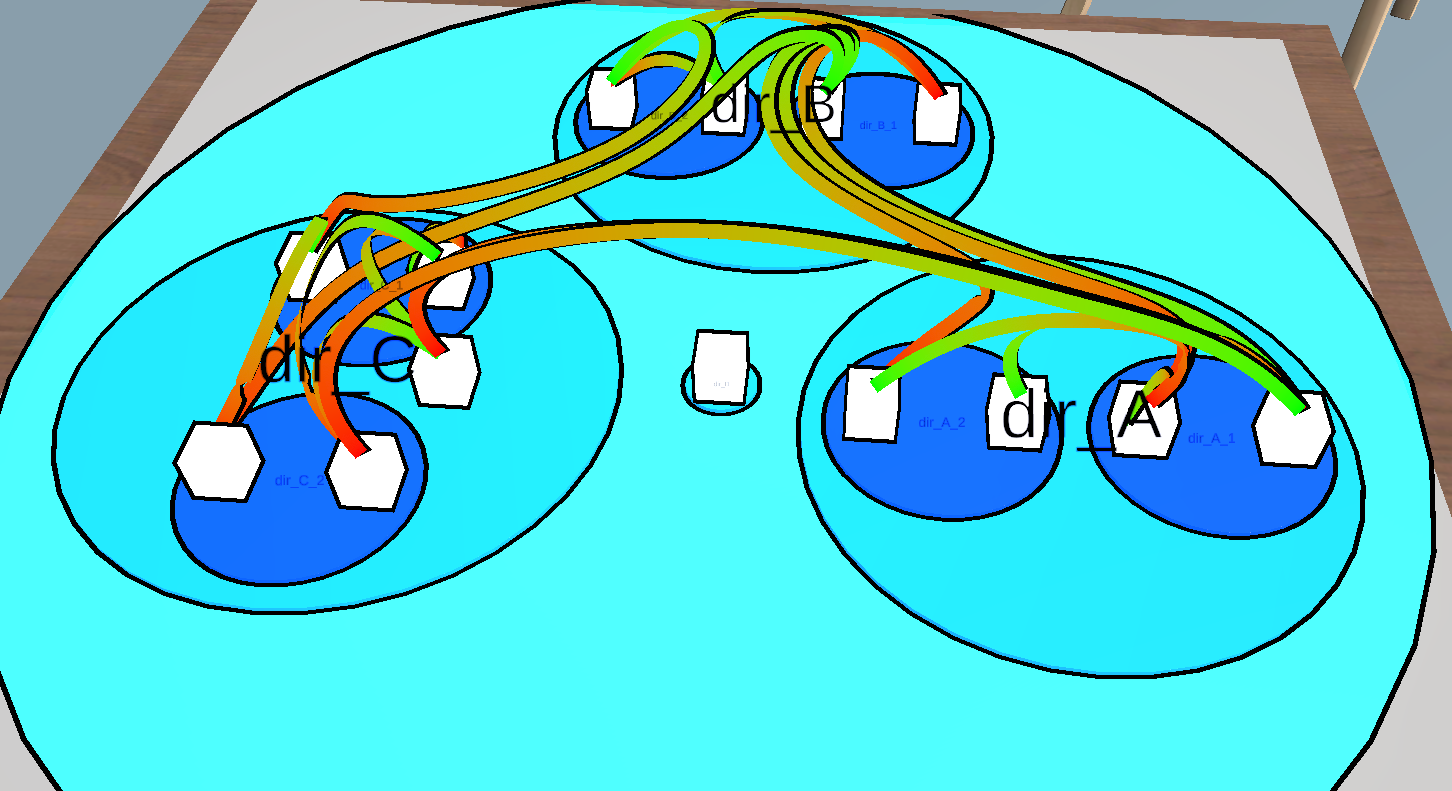
\includegraphics[width=1\textwidth]{Evaluation/img/city_1.png}
  \caption{The first \gls{city} for the user study}\label{fig:city1}
\end{figure}

\begin{figure}[H]
  \centering
  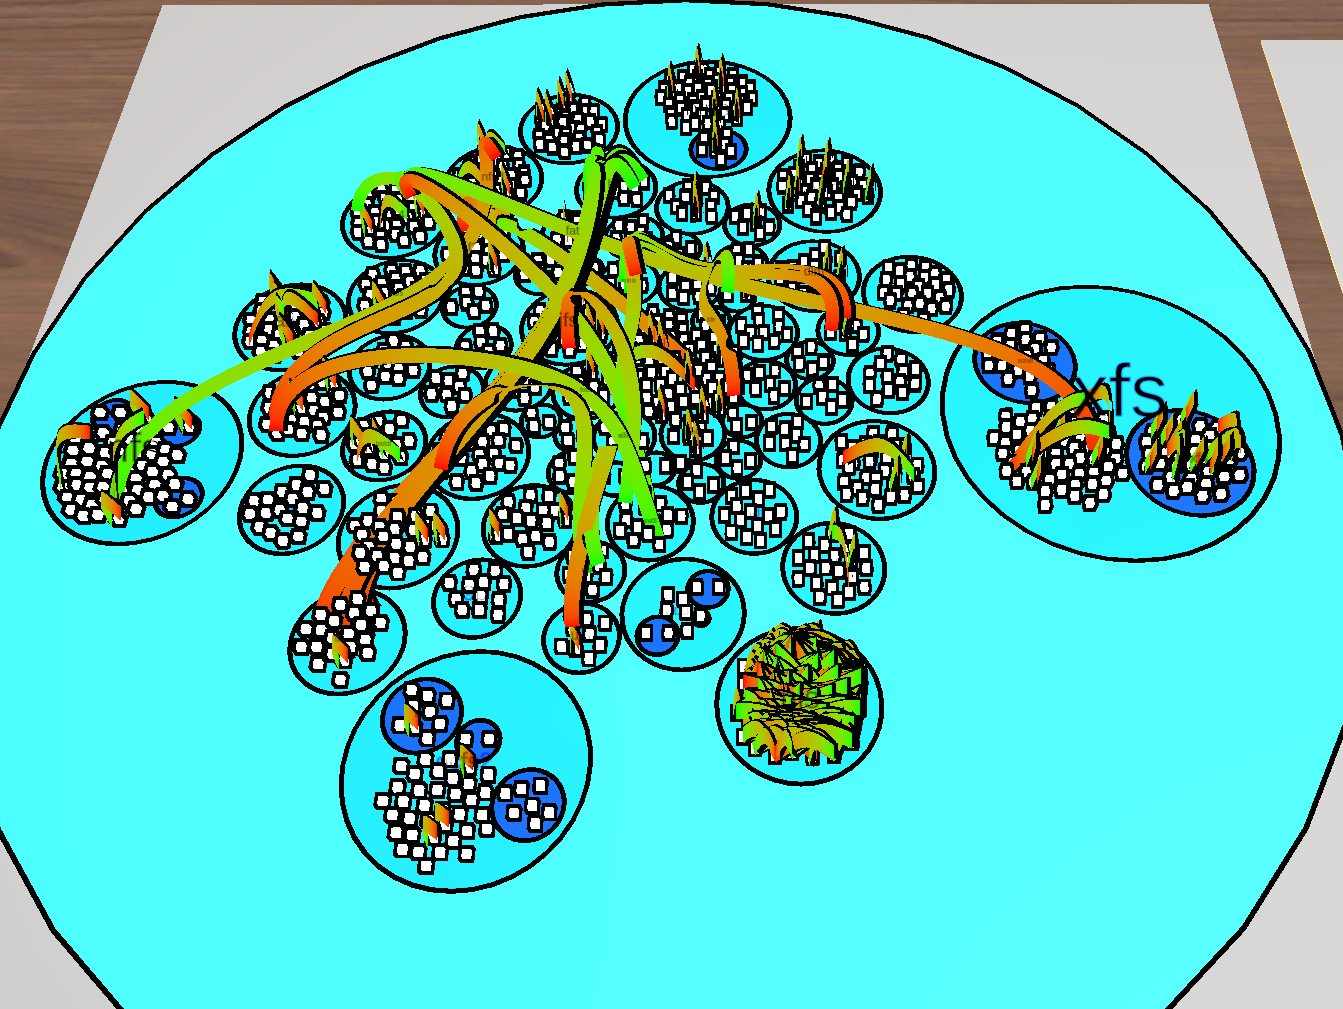
\includegraphics[width=1\textwidth]{Evaluation/img/city_2.png}
  \caption{The second \gls{city} for the user study}\label{fig:city2}
\end{figure}

\begin{figure}[htb]
  \centering
  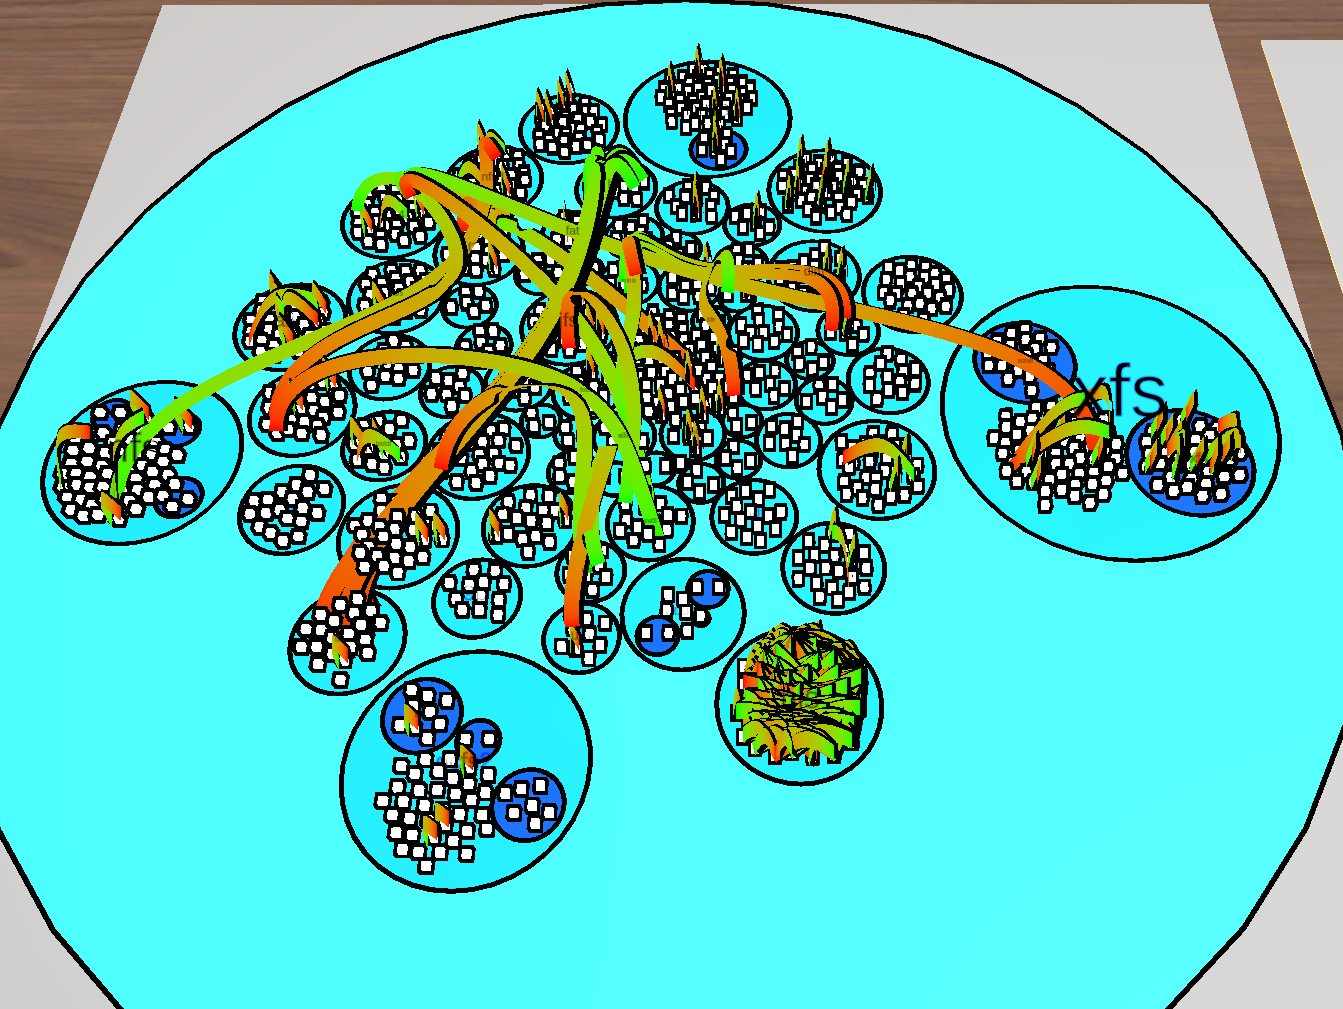
\includegraphics[width=1\textwidth]{Evaluation/img/city_3.png}
  \caption{The third \gls{city} for the user study}\label{fig:city3}
\end{figure}
In this survey the subjects will be asked various demographic questions as well as what \gls{android} device and version they will be using.
In addition to that the subjects will be asked if they are experienced with \gls{see} and if they are experienced with software development.
Before the subjects will be asked to solve various tasks they will be asked to watch a short tutorial video on each application.
After the video they will get a training task where every subject can get used to the system and ask questions if they have trouble solving the training task.
The overseer will also make sure that every essential action will be practiced such as zooming and moving the \gls{city}.
Figure \ref{fig:city1} shows a small arranged \gls{city} that shall be used for the training tasks.
The structure of the training \gls{city} is generic and follows a simple pattern.
That shall ensure that the user can focus on the training and that the user does not get overwhelmed.

Following the first questions and the training, the subjects can start with the main tasks.
For each application there will be two tasks and after each task the subjects will be handed a \gls{post-task} questionnaire.
Last but not least there will another questionnaire that aims to scale the \gls{usability} of the two applications.
For the \gls{post-task} questions the \gls{ASQ} will be used and for the \gls{usability} questions \gls{sus} will be used.
Both questionnaires will be discussed later on in section \ref{questionaires}.
For each main task the overseer will also take the completion time of every main task.
The first and second task on the first device will be performed on the \gls{city} that can be seen in figure \ref{fig:city2} and the third and forth task on device two will be performed on the \gls{city} that can be seen on figure \ref{fig:city3}.
These examples are much larger than the training \gls{city} and represent real life code.
The second \gls{city} shows the file system of Linux and the third one shows the network component of Linux.
That way the tasks might reflect better on real world uses for \gls{see}.

To not exhaust the testers too much the experiment shall not take longer than one hour.
This also ensures that there is no to little variance due to exhaustion.
Each participant might have a different concentration span, but this shall not be the focus of this experiment.

\subsection{Realization}
\label{real}
The following sections will cover the realization of the previously planned study. 
The choice of the used survey tool and questionnaires will be explained in section \ref{survey} and section \ref{questionaires}.
Afterwards a pilot study will be executed to test the study and possibly find missing aspects in section \ref{pilot}.
Finally, the final experiment set up will be discussed in section \ref{final}.

\subsubsection{Survey tool}
\label{survey}
As a survey tool Google Forms\footnote{https://www.google.com/forms/about/ (last visit: 05.06.2022)} will be used.
The survey tool has to fulfill the following requirements: 
\begin{itemize}
  \item The study will be online because an overseer has to attend every experiment, and therefore it comes in handy to be flexible in terms of location. For this reason the survey shall be fully in a browser. 
  \item The survey tool should be free to use.
  \item Subjects shall be anonymous.
  \item The results shall be exportable in a data format like \gls{csv}
  \item Subjects should have the option to presave their answers. In addition to that answers should not be lost on reload.
  \item There should be an option to embed the introduction videos in the survey.
\end{itemize}

Google Forms fulfills all these requirements and will therefore be used. 
The final form can be seen in figure \ref{fig:intro} which shows the intro of the survey and in figure \ref{fig:video} which shows the embedded intro video for \gls{see} mobile.
\begin{figure}[H]
  \centering
  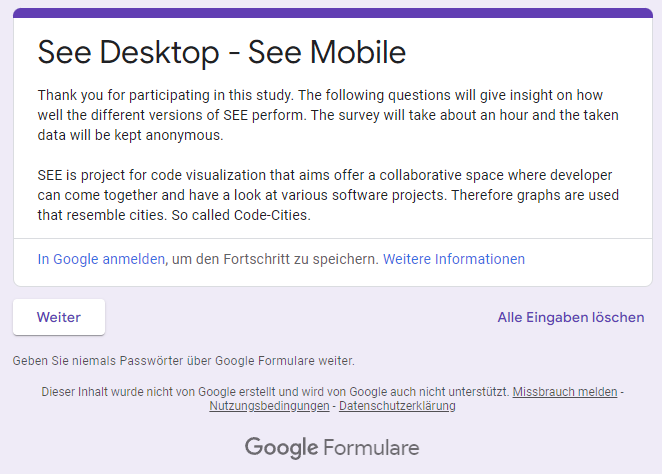
\includegraphics[width=1\textwidth]{Evaluation/img/form_intro.png}
  \caption{The intro of the survey}\label{fig:intro}
\end{figure}

\begin{figure}[H]
  \centering
  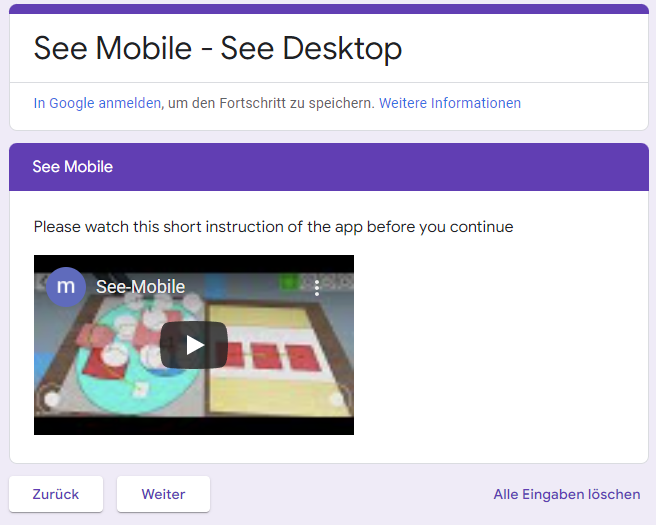
\includegraphics[width=1\textwidth]{Evaluation/img/form_video.png}
  \caption{The introduction video of the survey}\label{fig:video}
\end{figure}

\subsubsection{Questionnaires}
\label{questionaires}
There will be three questionnaires used for the study that will be discussed in detail in the following.
The study will start with a demographic questionnaire that covers general information about the subject.
After every task there will be \gls{ASQ} and after every block of tasks for each of the two covered devices there will be a \gls{sus} questionnaire.
\paragraph{Demographic questionnaire}\mbox{}\\
The subjects shall start the survey with a demographic questionnaire.
In that section they will be asked for their age, gender, the highest degree, experience with \gls{see}, experience with first person video games, their \gls{android} device name, their Android version and their experience with software development.
These specifications will be used to form different groups to see if there is any impact on the result of the following measurements. 
\cite{Mclellan2011} has shown that the user experience can have a significant impact on the \gls{sus}-score.
It is therefore important to view the measured results in context of the paired demographic data.

The mobile version was only tested on a single \gls{android} device.
It is likely that the performance of the application varies on different \gls{android} versions or devices.

\paragraph{Post-task questionnaire}\mbox{}\\
The \gls{post-task} questionnaire will supplement the \gls{post-study} questionnaire on a micro level.
The main focus here will be on single tasks, which allows to have a look at different aspects like effort, complexity and information provided by the system. 

As a \gls{post-task} questionnaire the \gls{ASQ} will be used. 
The \gls{ASQ} was first introduced in 1991 by \cite{lewis1991psychometric}.
It is designed for task based surveys and contains three questions.
The \gls{ASQ} will be used because it brings the following advantages:
\begin{itemize}
  \item The questionnaire has been used many times over the years and has proven its validly (\cite{hajesmaeel2022most}; \cite{lewis1991psychometric}; \cite{lewis1995ibm}).
  \item With its three questions it is short and does not exhaust the subjects. This is especially important because it will be required to finish this questionnaire a total of four times.
  \item It fits well for this study because it is a questionnaire designed for task based evaluations.
\end{itemize}
The \gls{ASQ} consists of three questions that scale from one to seven where one means \enquote{strongly disagree} and seven means \enquote{strongly agree}.

\paragraph{Post-study questionnaire}\mbox{}\\
The \gls{post-study} questionnaire is mainly to obtain as much information about the \gls{usability} of the two systems as possible.
The questionnaire can be longer than the \gls{post-task} but still should not be to long to keep the processing time of the survey at around an hour.

The \gls{sus} questionnaire was first published in 1986 by John Brooke (\cite{brooke1996sus}) and is therefore widely used and proven as citations in more than 1200 publications up until 2013 show (\cite{brooke2013}).
The \gls{sus} is used in this study for the following advantages: 
\begin{itemize}
  \item It consists of ten questions and has to be done two times. Twenty questions in total fit well into the planned one hour total time span of this experiment.
  \item It has been made publicly available and is free to use (\cite{brooke1996sus}).
  \item It is widely used and therefore already proven to give useful results (\cite{brooke2013}; \cite{lewis2018system}; \cite{grier2013system}).
  \item According to \cite{doi:10.1177/1541931213571043} and \cite{doi:10.1080/10447310802205776} it is suited to compare two systems.
\end{itemize}
The \gls{sus} questionnaire will contain as already mentioned ten questions.
Each question will give a five-level rating from \enquote{strongly disagree} to \enquote{strongly agree}.
The results will then be combined into a \gls{usability}-score from zero to 100 where a high value represents a good result and a low value a bad one.
\subsubsection{Pilot study}
\label{pilot}
In a first test the pilot study was executed with one subject.
Afterwards the study was discussed and checked for errors.
It stood out that the example \gls{city} of task one was too different to the one in the second task.
Therefore, the \gls{city} of the first task was exchanged with a larger and better comparable one.
Further on a \gls{city} with 1288 nodes (see figure \ref{fig:city2}) as well as one with 1464 nodes (see figure \ref{fig:city3}) will be used.

\begin{figure}[htb]
  \centering
  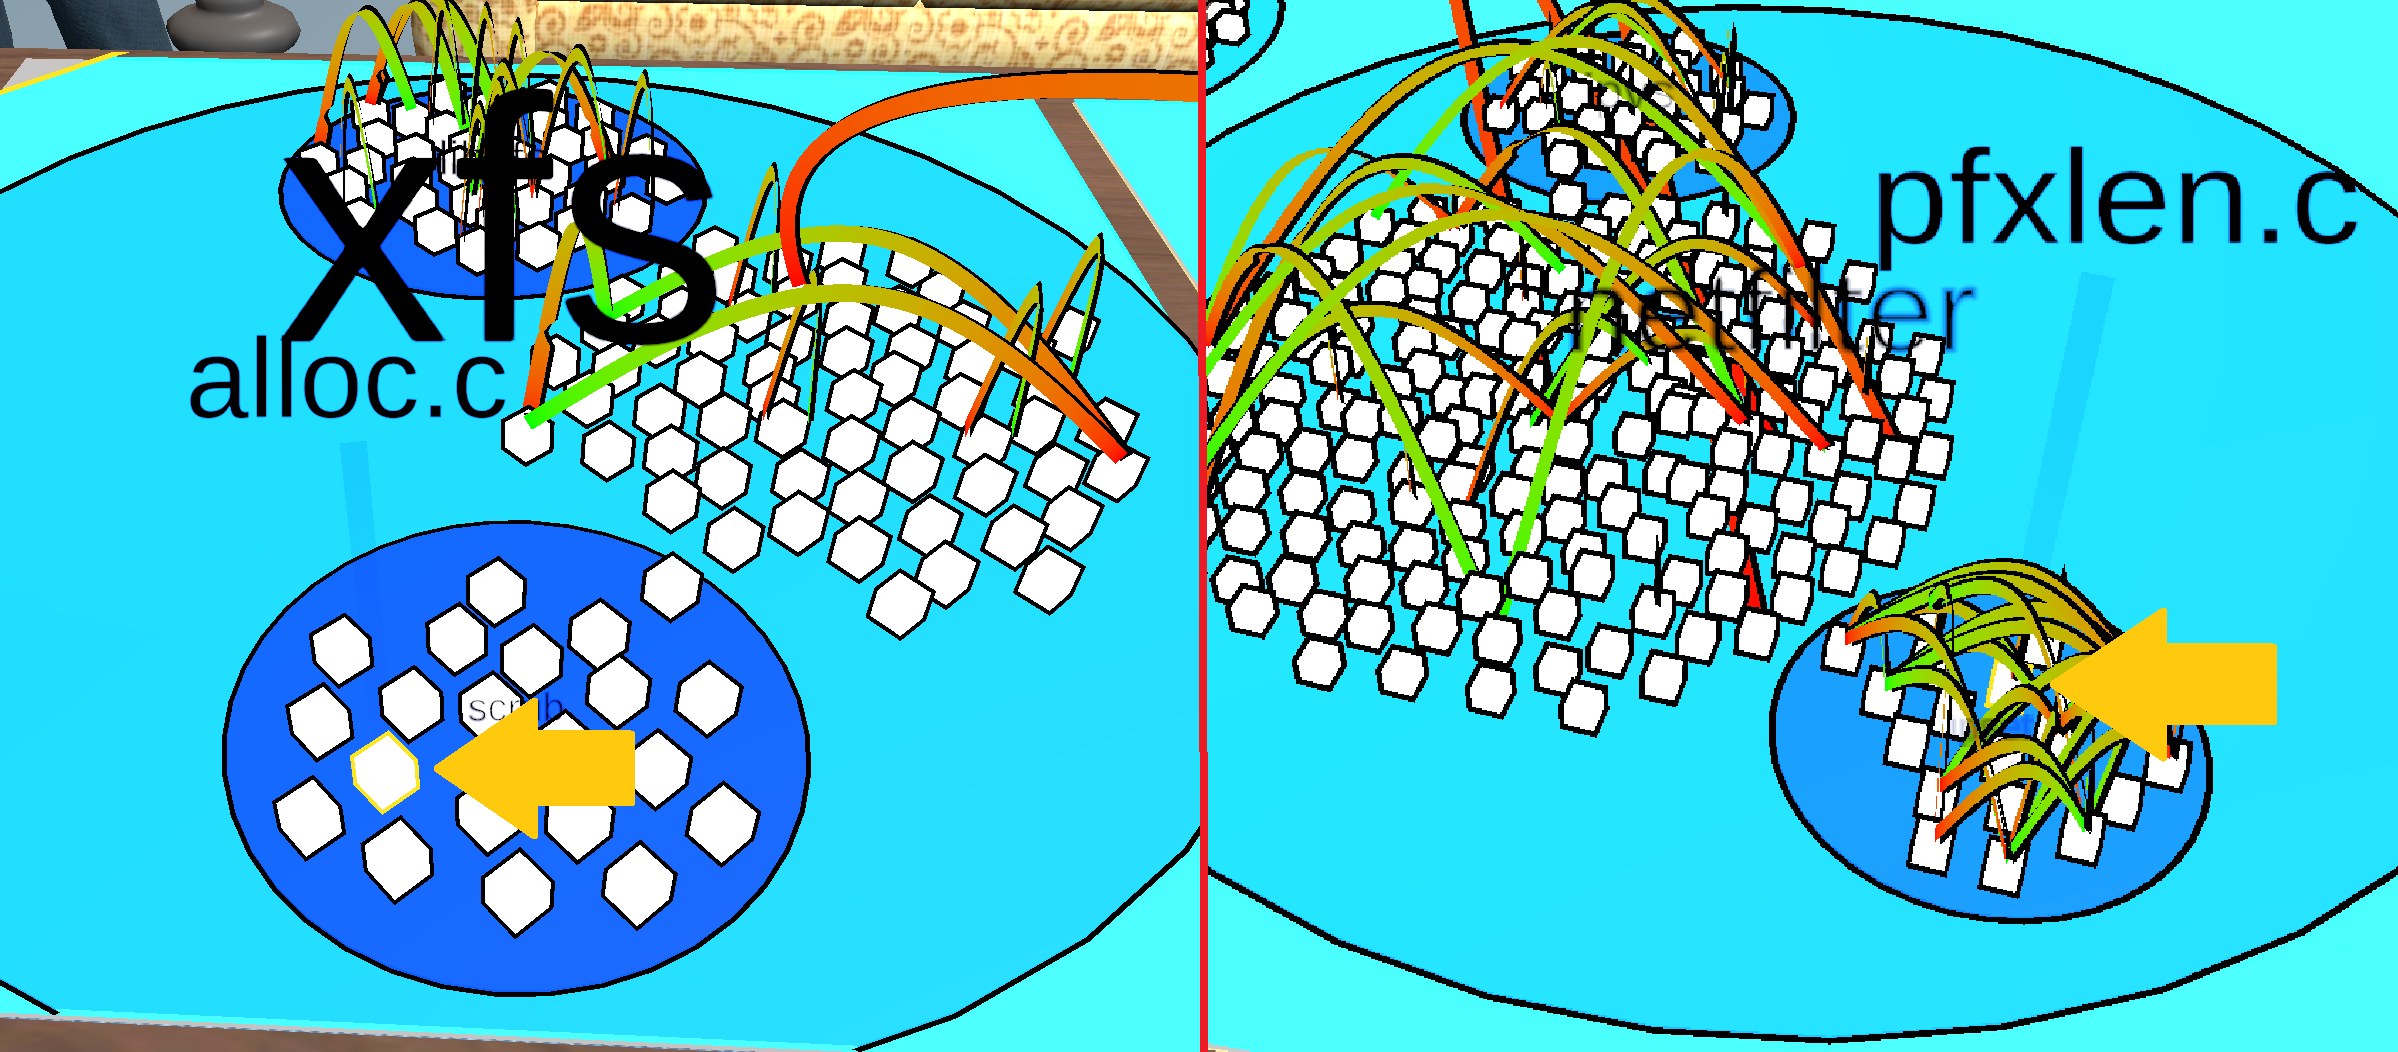
\includegraphics[width=1\textwidth]{Evaluation/img/task1.png}
  \caption{The two key nodes are marked with a yellow arrow}\label{fig:task1}
\end{figure}

Also, the tasks were not comparable because they differed in the types of interactions they used.
In one task the user was asked to rename a node and in the other one the user shall add four nodes.
For renaming a node the user has to use a keyboard which does not make it comparable to just click and add nodes in the second task.

To also ensure that task one and task three (first task of each version) were comparable both task are similar in their set-up as seen in figure \ref{fig:task1}.
As one part of the task is to find the right node both are on a plane with a similar amount of nodes.

The same goes for task three and four (second task of each device) as the target planes that have to be found have a similar size. 
Both tasks also include a hint where to find the desired planes.

\subsubsection{Final experiment set-up}
\label{final}
After the pilot study the final set-up can be discussed.
The demographic questionnaires will be designed as described in section \ref{experiment}.
The final questions will be as listed below.
\paragraph{Demographic questions:}
\begin{itemize}
  \item Age
        \begin{itemize}
          \item 0-15 years old
          \item 16-30 years old
          \item 31-45 years old
          \item 46+ years old
        \end{itemize}
  \item What gender do you identify as?
        \begin{itemize}
          \item Male
          \item Female
          \item Other ...
          \item Prefer not to say
        \end{itemize}
  \item What is the highest degree or level of education you have completed?
        \begin{itemize}
          \item Some High School (Hauptschule/Realschule...)
          \item High School (Abitur)
          \item Bachelor's Degree
          \item Master's Degree
          \item Ph.D. or higher
          \item Prefer not to say
          \item Other ...
        \end{itemize}
  \item Questions regarding used hardware and experience
        \begin{itemize}
          \item Are you already experienced with See?
          \item Do or did you play first person video games?
          \item Do or did you develop software?
          \item On which \gls{android} device will you attend?
          \item Which \gls{android} version are you using?*
        \end{itemize}
\end{itemize}

After filling out the demographic questionnaires the subjects will be asked to watch a short tutorial video.
Which video they will watch first will depend on with group they are in.
If they start with the mobile version of \gls{see} they will be asked to watch \hyperref[calc]{SeeMobile.mp4} otherwise they will be asked to watch \hyperref[calc]{SeeDesktop.mp4}.
After completing their first training and their first two tasks, as described in table \ref{table:tasks}, they will be asked to watch the video they have not started with.

\begin{table}[htb]
  \resizebox{\textwidth}{!}{%
    \begin{tabular}{lll}
      Nr.                                                                                                                                                                                         &
      Task                                                                                                                                                                                        &
      Expected time                                                                                                                                                                                 \\ \hline
      Training                                                                                                                                                                                    &
      \begin{tabular}[c]{@{}l@{}}Navigate through the planes "dir\_root" \\ \textgreater "dir\_B" \textgreater "dir\_B\_2". On that plane \\ select "b2\_b.cpp" and rename it "b42".\end{tabular} &
      1 - 5 mins                                                                                                                                                                                    \\
      1                                                                                                                                                                                           &
      \begin{tabular}[c]{@{}l@{}}Detect the largest plane "xfs". On that\\ plane find plane "scrub". Then find \\ and delete node "alloc.c".\end{tabular}                                         &
      0.5 - 5 mins                                                                                                                                                                                  \\
      2                                                                                                                                                                                           &
      \begin{tabular}[c]{@{}l@{}}Find the plane with one blue child \\ plane ("btrfs"). On the blue child \\ plane "tests" add four new nodes.\end{tabular}                                       &
      1 - 5 mins                                                                                                                                                                                    \\ \hline
      Training                                                                                                                                                                                    &
      \begin{tabular}[c]{@{}l@{}}Navigate through the planes "dir\_root" \\ \textgreater "dir\_C" \textgreater "dir\_C\_2". On that plane \\ select "c2\_b.cpp" and rename it "c42".\end{tabular} &
      1 - 5 mins                                                                                                                                                                                    \\
      3                                                                                                                                                                                           &
      \begin{tabular}[c]{@{}l@{}}Detect the \\ largest plane "netfilter". On that plane\\ find plane "ipset". Then find and \\ delete node "pfxlen.c".\end{tabular}                               &
      0.5 - 5 mins                                                                                                                                                                                  \\
      4                                                                                                                                                                                           &
      \begin{tabular}[c]{@{}l@{}}On the plane with the most \\ edges ("ipv6") find the smallest plane\\ "ila" and connect all four nodes on it.\end{tabular}                                      &
      1 - 5 mins                                                                                                                                                                                    \\ \hline
    \end{tabular}%
  }
  \caption{The tasks used for the experiment. The device will be switched after task 2.}
  \label{table:tasks}
\end{table}

After each task the subjects will be asked to fill out a \gls{ASQ} and after each block of task, as described in table \ref{table:procedure}, they will be asked to fill out a \gls{sus} questionnaire.
Therefore, each participant has to fill out four \glspl{ASQ} and two \gls{sus} questionnaires.
The full study should not take longer than an hour.

\begin{table}[htb]
  \resizebox{\textwidth}{!}{%
    \begin{tabular}{llll}
      Phase          &                        & \multicolumn{2}{l}{Description}                                          \\ \hline
      Pre-Experiment &                        & \multicolumn{2}{l}{Demographic questionnaire}                            \\ \hline
                     & City                   & Group 1                                       & Group 2                  \\ \hline
      Training       & Figure \ref{fig:city1} & \multirow{6}{*}{Desktop}                      & \multirow{6}{*}{Mobile}  \\
      Task 1         & Figure \ref{fig:city2} &                                               &                          \\
      ASQ            &                        &                                               &                          \\
      Task 2         & Figure \ref{fig:city2} &                                               &                          \\
      ASQ            &                        &                                               &                          \\
      SUS            &                        &                                               &                          \\ \hline
      Training       & Figure \ref{fig:city1} & \multirow{6}{*}{Mobile}                       & \multirow{6}{*}{Desktop} \\
      Task 3         & Figure \ref{fig:city3} &                                               &                          \\
      ASQ            &                        &                                               &                          \\
      Task 4         & Figure \ref{fig:city3} &                                               &                          \\
      ASQ            &                        &                                               &                          \\
      SUS            &                        &                                               &
    \end{tabular}%
  }
  \caption{Experimental procedure per subject. The procedure is swapped per group.}
  \label{table:procedure}
\end{table}


\subsubsection{Execution}
Before the study the subjects got an installation instruction as well as the two applications.
For the execution of the user study every subject got one of two links to a Google form.
Each form starts with a different device. 
The forms were handed out in alternating order and the subjects should therefore be assigned random to the two groups.

The study was executed within a week and a total of 20 subjects participated.
From the 20 subjects, two could not finish the tasks on their mobile device, which leaves n = 18 participants that finished the survey.

The overseer hosted an instance of \gls{see} from his home network and watched the subjects doing their task.
He also gave instructions for the training tasks and made sure that all essential interactions were trained such as zooming and moving the \gls{city}.
Every subject got the same training.


\subsection{Results}
The \hyperref[calc]{calc\_data.ipynb} script can be used to reproduce the result data for the following section.
Also, all shown diagrams in this section can be reproduced with the script.

In the following the group that started the study with the desktop version of \gls{see} will be called \textit{Group 1} and the group starting with the mobile version will be called \textit{Group 2}.
The task order of the two groups remains the same.
Both groups start with the same task.
That way not only both groups but also the desktop and the mobile \gls{see} version will be compared. 

In the coming up section the \gls{utest} will be used multiple times to see if there are significant differences between to data sets.
The \gls{utest} brings the advantage that the tested data sets do not need to fulfill the requirement of a normal distribution (\cite{gibbons1991comparisons}).
This is important because the sample size of n = 18 is too small to assume a normal distribution.
The used level of significance will be $\alpha = 0.05$.

\label{results}
\subsubsection{Demographic data}
\label{sec:demo}
In this subsection it will be verified if the two groups differ significantly in their demographic data. 
Therefore, a two-tailed \gls{utest} that checks whether a set of demographic values from \textit{Group 1} $\neq$  a set of demographic values from \textit{Group 2} will be used.
Both groups have a sample size of $n = m = 9 $ with $\alpha = 0.05$ which leads to a critical value of $U = 17$ for a two-tailed \gls{utest} (\cite{zar2010biostatistical}).

\paragraph{Gender}\mbox{}\\
Of 18 participants, 17 reported being male. 
One participant preferred not to say his or her gender and can therefore not be grouped.
Due to this fact a grouping does not make sense here in general. 

\paragraph{Age}\mbox{}\\
The subjects were asked to choose their age in grouped options. 
Most of the participants were aged between 16 and 30 years.
Only two participants were aged between 31 and 45 years. 
Therefore, the age of the participants should not fall into account of the results of the study.

\paragraph{Highest degree}\mbox{}\\
Nine of the participants answered with \enquote{Bachelor's Degree} for their highest achieved degree. 
It is therefore the most common option as pictured in figure \ref{fig:degree}.

To measure the \gls{utest} the options were put into an ordinal scale which follows the same order as in the survey.
The test shows there is no significant difference between the two groups ($U = 33.0; p \approx 0.51$).

\begin{figure}[H]
  \centering
  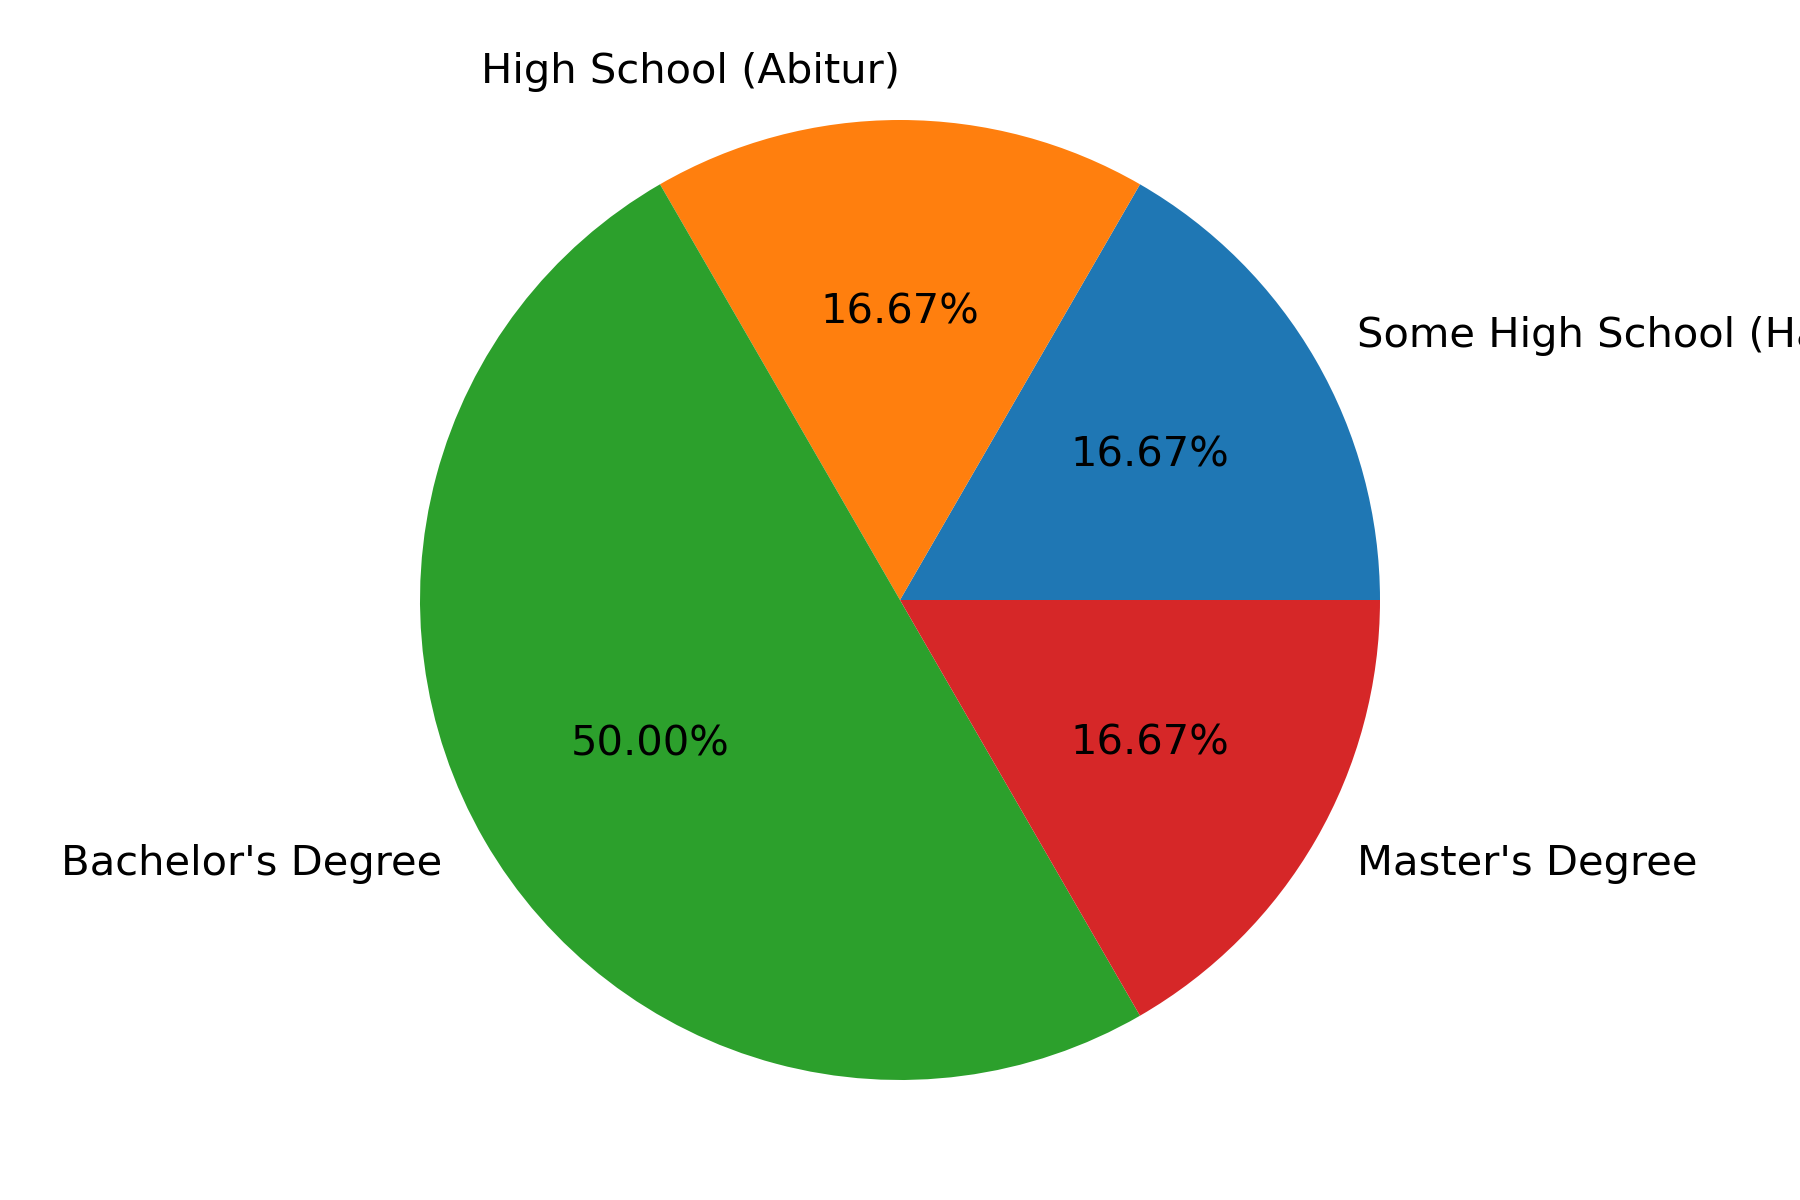
\includegraphics[width=0.7\textwidth]{Evaluation/img/degree.png}
  \caption{The distribution of the highest completed degrees of all 18 subjects}\label{fig:degree}
\end{figure}

\paragraph{Experience}\mbox{}\\
The subjects were asked if they had experience regarding \gls{see}, software development and first person video games.
All but one subject had experience with first person video games and the single subject without experience had at least experience with \gls{see} which could arguably count as a first person video game.
Therefore, experience with first person video games should not have an impact on this study.

Five of 19 subjects had experience with \gls{see}.
The \gls{utest} shows there is no significant difference between the two groups ($U = 27.0; p \approx 0.23$).
Even though there is no significant difference, four of the subjects with \gls{see} experience are in \textit{Group 2} and only one in \textit{Group 1}.

The majority of ten subjects had experience with software development.
The other eight subject had no experience.
The \gls{utest} shows there is no significant difference the two groups ($U = 49.5; p \approx 0.38$).

\paragraph{Android device and version}\mbox{}\\
A large variety of 17 different \gls{android}d devices were used.
Therefore, the distribution of \gls{android} devices should not have impact on the study results.
Nonetheless, it has to be considered that the devices \enquote{Huawei P10 lite}, \enquote{Huawei P20 Pro} \enquote{Samsung A52S}, \enquote{Samsung S9} and the \enquote{Poco X3 Pro} had performance issues.
These performance issues showed in bumpy movement and player interactions.
Unfortunately, it could not be measured how strong the impact was on the performance on the single phones.
The threads of validity this could cause will be further discussed in section \ref{sec:validity}.
Three of the devices with bad performance belong to \textit{Group 1} and the other two to \textit{Group 2}.

The \gls{android} version was not distributed as much as the \gls{android} devices used. 
The most common used one was \gls{android} 12, which is also the most current one to the time of this writing.
\gls{android} 12 was used by seven subjects.
The second most used version was \gls{android}d 11.
One subject used \gls{android} 7 on the \enquote{Huawei P10 lite}.
Which is remarkable because \gls{android} 7 was released in 2016\footnote{\url{https://android-developers.googleblog.com/2016/08/taking-final-wrapper-off-of-nougat.html} (10.06.2022, 12:37)} and the \enquote{Huawei P10 lite} was released a little later in March 2017\footnote{\url{https://www.gsmarena.com/huawei_p10_lite-8598.php} (10.06.2022, 12:37)} but \gls{see} still managed to work, if with lower performance.
The distribution of the used \gls{android} devices can be seen in \ref{fig:android_version}.
The \gls{utest} shows there is no significant difference the two groups ($U = 39.0; p \approx 0.93$).

\begin{figure}[htb]
  \centering
  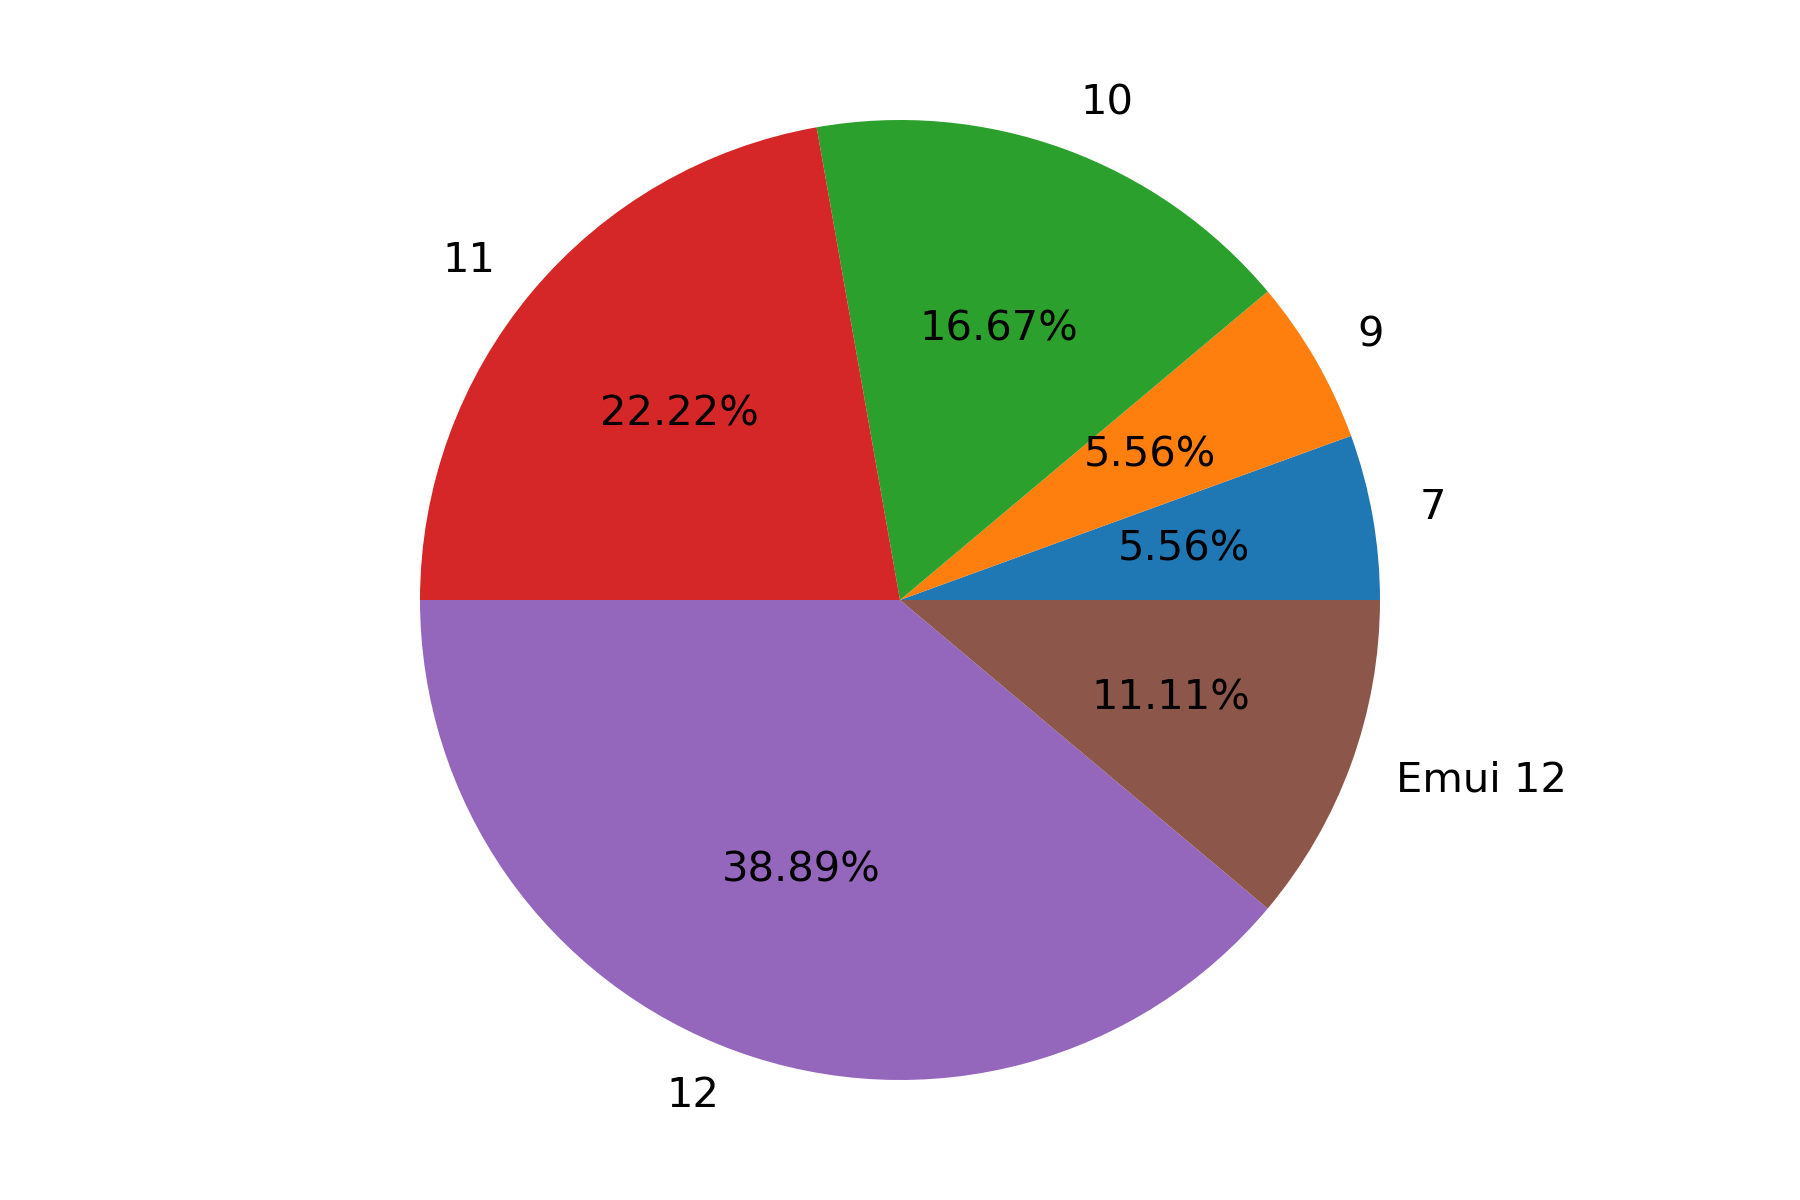
\includegraphics[width=0.7\textwidth]{Evaluation/img/droid_version.png}
  \caption{The distribution of the Android versions the subjects were using}\label{fig:android_version}
\end{figure}

\mbox{}\\
Surprisingly there has been no significant difference with the demographic data between the two groups.
In the following section the more exciting data will be analyzed. 

\subsubsection{Performance}
For the performance the time needed for each task was measured.
The time for the trainings task, however, was not measure because it would not fit the purpose of a training to be measured by time.
Therefore, the overseer asked the subjects to tell him when they begin the task. 
The time was taken after the subject has read and understood the task, and it was stopped when the subject successfully finished.
This will help to prove or discard hypothesis $H_{a}$.

Let's have a look at the two groups in general.
Is there any significant difference?
The total time needed for all subjects in the two groups can be seen in figure \ref{fig:group_time_violin}.
The average time \textit{Group 1} needed to complete all tasks was $\overline{t_1} = 487s$ and for \textit{Group 2} it was $\overline{t_2} = \approx388s$.
The median time for \textit{Group 1} was $\widetilde{t1} = 315s$ and for \textit{Group 2} it was $\widetilde{t_2} = 384s$.
As figure \ref{fig:group_time_violin} and the values mentioned above suggest the \gls{utest} shows there is no significant difference between the two groups with a $U = 43.0$ and $p \approx 0.86$.

\begin{figure}[htb]
  \centering
  \includegraphics*[width=1\textwidth]{Evaluation/img/group_time_violin.png}
  \caption{Total time each group needed as violin plot}
  \label{fig:group_time_violin}
\end{figure}

Furthermore, let's look at the single tasks. 
Has there maybe been a learning effect or difference in general between the groups? 
To find out task 1 from \textit{Group 1} will be compared with task 3 from \textit{Group 2} and so on.
Every couple of tasks is comparable because they have been done on the same device and use the same set of user interactions as described in section \ref{final}.
The \gls{utest} shows that there is no significant difference in any combination as listed below:
\begin{itemize}
  \item \textit{Group 1}, task 1 \& \textit{Group 2}, task 3: $U = 26.5; p \approx 0.23$
  \item \textit{Group 1}, task 2 \& \textit{Group 2}, task 4: $U = 35.5; p \approx 0.69$
  \item \textit{Group 1}, task 3 \& \textit{Group 2}, task 1: $U = 49.0; p \approx 0.48$
  \item \textit{Group 1}, task 4 \& \textit{Group 2}, task 2: $U = 57.0; p \approx 0.16$
\end{itemize}

Finally, let's see if there is a significant difference between the two used versions of \gls{see} in the single tasks.
The time needed for every single task on both versions can be seen in figure \ref{fig:speed_violin}.
There are some results that stand out and took way longer than the medians would suggest.
That could be caused by various reasons as for example:
\begin{itemize}
  \item The mobile version of \gls{see} did not run smooth on the subjects device and therefore the tasks became harder.
  \item The subject did not understand the task correctly and has to reread it.
  \item The subject overlooked a key object and continued the search at wrong areas.
\end{itemize}

\begin{sidewaysfigure}
  \centering
  \includegraphics*[width=1.15\textwidth]{Evaluation/img/speed1_violin.png}
  \caption{Violin plots of all tasks by device}
  \label{fig:speed_violin}
\end{sidewaysfigure}

To prove the hypothesis, $H_a$ for every task will be checked if the subjects needed significantly less time with the desktop version of \gls{see} than with the mobile version.
Therefore, a one-sided \gls{utest} will be used.
The critical value here is $U = 21$.

\begin{description}
  \item[Task i] The subjects needed an average time of $\approx 80s$ with the desktop version and $\approx 166s$ with the mobile version. 
  The median here was 47s with the desktop version and 150s with the mobile version. 
  The medians show that there are son outliers on both sides that took longer than the usual subject needed. 
  The one-sided \gls{utest} shows, with $U = 19; p \approx 0.03$, that the subjects needed significantly less time than with the mobile version.
  \item[Task ii] This task shows the lowest notable difference in figure \ref{fig:speed_violin}. 
  The \gls{utest} shall confirm this assumption with $U=24; p \approx 0.08$.
  This results that the subjects did not need significantly less time to solve task 2 with the desktop version than with the mobile version.
  The average time of the desktop version here is $\approx 47s$ and of the mobile version $\approx 74$, while the desktop median lays at $57s$ and the mobile median at $67s$.
  \item[task iii] In contrast to task 2 this task shows the biggest difference in figure \ref{fig:speed_violin} and once again the one-sided \gls{utest} approves this clearly with a result of $U=12.0;p \approx 0.007$. 
  This shows that the desktop version needed significantly less time than the mobile version once more. 
  Also, the average time needed spread quite far with an average of $\approx 82s$ for the desktop version and $\approx 247s$ for the mobile version.
  The median values are 77s for the desktop version and 151s for the mobile version.
  The desktop median is almost the same as the desktop average while the mobile median is again quite far from the average, which shows that there are again some outliers that took much longer than the usual subject. 
  This could, among other things, be caused by the reported bad performance of the devices \enquote{Huawei P20 Pro} and \enquote{Huawei P10 Lite}, which were used for task 3.
  \item[Task iv] The average time needed to complete the task was $\approx 67s$ for the desktop version and $\approx 113s$ for the mobile version. 
  The medians here were 46s for the desktop version and 111s for the mobile version. 
  The values differ quite much and the \gls{utest} validates one last time that the desktop version needed significantly less time than the mobile version to complete the tasks ($U=17.5;p \approx 0.023$).
\end{description}

To close this section figure \ref{fig:device_time_violin} shows the total time needed for all tasks by used device.
The one-sided \gls{utest} for the null hypothesis has a clear result of $U=11.0$ and $p \approx 0.005$.
Therefore, the null hypothesis $H_a0:$ \enquote{The time required in \gls{see} desktop is higher
or the same as the time required in see mobile} can be rejected, and the alternative hypothesis can be assumed true.

\begin{figure}[htb]
  \centering
  \includegraphics*[width=1\textwidth]{Evaluation/img/device_time_violin.png}
  \caption{Total time the subjects needed on the different devices as violin plot}
  \label{fig:device_time_violin}
\end{figure}

Summarized it can be said that the subjects were faster on the desktop version of \gls{see}.
All data sets regarding the required time to solve the four tasks are comparable even crossed over like for example task 1 and task 3. 
Only for one task the subjects did not need significantly less time on the desktop version, but the border value to a significant result was quite close.
All in all the desktop version did perform better than the mobile version regarding the required time.

\subsubsection{Usability}
\label{sec:usability}
This section will discuss the results of the usability questionnaires presented in section \ref{questionaires}.
First the \gls{ASQ} results will be analyzed and second the \gls{sus} results to test the hypotheses presented in section \ref{aim}.
\paragraph{ASQ}\mbox{}\\
As a start the \gls{post-task} questionnaire will be looked at. 
Figure \ref{fig:asq_group} shows the ASQ results by group independent of the used device.
Unfortunately the result differ significantly as the \gls{utest} shows with $U=392.5$ and $p \approx 0.0037$.
Therefore, a deeper look is needed. 
The results of \textit{Group 1} do not differ significantly from \textit{Group 2} looking only at the tasks completed with the desktop device as the \gls{utest} shows with $U=122.5$ and $p \approx 0.21$.
On the other hand side the results only caused by completing tasks with a mobile device differ significantly as the \gls{utest} shows ($U=73.0;p \approx 0.0048$).
Having another look at figure \ref{fig:asq_group} the result on \textit{Group 1} only on the mobile stands out. 
Comparing the two groups without the described results of \textit{Group 1} results in a \gls{utest} of $U=266.5; p \approx 0.29$, which means without the subset of \textit{Group 1} the two groups show no significant difference.

\begin{sidewaysfigure}
  \hspace*{-1.5in}
  \centering
  \includegraphics*[width=1.15\textwidth]{Evaluation/img/group_asq_violin.png}
  \caption{Violin plots of all tasks by group}
  \label{fig:asq_group}
\end{sidewaysfigure}

To ensure a good comparability further on the all task will be looked at separately. 
The \gls{ASQ} consists of three questions.
Each representing a different aspect.
In the following all tasks will be compared as shown in table \ref{table:asq_combi}.

\begin{table}[htb]
  \resizebox{\textwidth}{!}{%
  \begin{tabular}{lllll}
    ASQ Question                        & \multicolumn{4}{l}{Complexity}  \\ \hline
    \multicolumn{1}{l|}{Group 1, Task:} & 1       & 2     & 3     & 4     \\
    \multicolumn{1}{l|}{Group 2, Task:} & 3       & 4     & 1     & 2     \\
    \multicolumn{1}{l|}{Mann-Whitney-U} & $U=47 ;p \approx 0.58$ & $U=37.5;p \approx 0.81$ & \cellcolor[HTML]{FFFC9E} $U=7.0;p \approx 0.003$  & $U= 24.5;p \approx 0.16$      \\ \hline
    ASQ Question                        & \multicolumn{4}{l}{Effort}      \\ \hline
    \multicolumn{1}{l|}{Group 1, Task:} & 1       & 2     & 3     & 4     \\
    \multicolumn{1}{l|}{Group 2, Task:} & 3       & 4     & 1     & 2     \\
    \multicolumn{1}{l|}{Mann-Whitney-U} & $U= 44;p \approx 0.78$        & $U=37 ;p \approx 0.78$      & \cellcolor[HTML]{FFFC9E} $U= 13.5;p \approx 0.02$      & $U= 23;p \approx 0.11$      \\ \hline
    ASQ Question                        & \multicolumn{4}{l}{Information} \\ \hline
    \multicolumn{1}{l|}{Group 1, Task:} & 1       & 2     & 3     & 4     \\
    \multicolumn{1}{l|}{Group 2, Task:} & 3       & 4     & 1     & 2     \\
    \multicolumn{1}{l|}{Mann-Whitney-U} & $U= 39.5;p \approx 0.96$ & $U= 36;p \approx 0.70$      & $U= 20.5;p \approx 0.07$      & $U= 20.5;p \approx 0.07$     
    \end{tabular}%
  }
  \caption{Two-sided \gls{utest} for each comparable question on the same device}
  \label{table:asq_combi}
  \end{table}

The two marked \glspl{utest} in table \ref{table:asq_combi} as they show that the pair \textit{Group 1, Task 3 - Group 2, Task 1 - ASQ Question 1} as well as \textit{Group 1, Task 3 - Group 2, Task 1 - ASQ Question 2} have significant differences.
As those two pairs are not comparable, they will not be observed further on.
All remaining results can be seen in figure \ref{fig:effort_violin} for the ASQ aspect effort, in figure \ref{fig:complexity_violin} for ASQ aspect complexity as well as in figure \ref{fig:info_violin} which covers the \gls{ASQ} aspect information.

\begin{figure}[htb]
  \hspace*{-1.4in}
  \centering
  \includegraphics*[width=1.4\textwidth]{Evaluation/img/effort_violin.png}
  \caption{ASQ effort results violin plots of all tasks by device}
  \label{fig:effort_violin}
\end{figure}

\begin{figure}[htb]
  \hspace*{-1.4in}
  \centering
  \includegraphics*[width=1.4\textwidth]{Evaluation/img/complexity_violin.png}
  \caption{ASQ complexity results violin plots of all tasks by device}
  \label{fig:complexity_violin}
\end{figure}

\begin{sidewaysfigure}
  \hspace*{-1.5in}
  \centering
  \includegraphics*[width=1.15\textwidth]{Evaluation/img/information_violin.png}
  \caption{ASQ information results violin plots of all tasks by device}
  \label{fig:info_violin}
\end{sidewaysfigure}

The \gls{utest} only shows significant findings for two tasks:
\begin{description}
  \item[Task iii] The desktop version of \gls{see} has significant better results than the mobile version in the aspect of information. 
  The subjects rated the desktop version with an average score of 6.22 and a median score of 7, while the mobile version was rated an average of 6.44 and a median of 5.22.
  The \gls{utest} results here are $U = 20.5$ and $p \approx 0.037$.
  \item[Task iv]  The desktop version also showed better results for the aspect of information in this task. 
  The subjects rated the desktop version with an average score of 6.44 and a median of 7, while the mobile version was rated with an average of 5.22 and a median of 6. 
  The \gls{utest} resulted in $U=20.5$ and $p \approx 0.035$ in a one-sided test, which means the desktop version got a significantly higher rating than the mobile version.
\end{description}

All other tasks show significant higher or lower results. 
It is also to mention that only the desktop version only scored a significant higher value at the aspect of information.
That was to be expected because the mobile versions offer less information because of its constrains regarding the screen size. 
The mobile version uses for example only icon button and not text buttons like the desktop version, which safe screen space but sacrifices information value since the user has to remember the meaning of each icon.

Finally, the hypotheses $H_b$, $H_c$, $H_d$ can be rated:

\begin{description}
  \item[$H_b$] The null hypothesis $H_{b0}$ can not be rejected since the \gls{utest} results in $U = 362.0; p \approx 0.23$. 
  Therefore, the alternative hypothesis can be assumed true, which means that the desktop score for the \gls{ASQ} aspect \textit{complexity} is not significantly higher. 
  \item[$H_c$] The same goes for null hypothesis $H_{c0}$. 
  It can not be rejected since the \gls{utest} results in $U = 348.5; p \approx 0.32$.
  That means that the desktop \gls{ASQ} score for the aspect \textit{effort} is also not significantly higher than the mobile \gls{ASQ} score.
  \item[$H_d$]  Two of the four tasks showed a significantly higher score for the desktop version in the \gls{ASQ} aspect \textit{information} but for all four tasks combined the null hypothesis $H_{d0}$ can not be rejected since the \gls{utest} resulted $U = 776.5; p \approx 0.06$.
  Although the results are much closer to the significance level of $\alpha = 0.05$ in this example.
 \end{description}

 The final ASQ scores, which are an average of all three questions, can be found in table \ref{table:asq}.
 However, the final ASQ-Scores still differ significantly as the \gls{utest} of $U=92.0; p \approx 0.03$ shows.
 Since, even after not taking into account the previously discussed pairs of tasks, the \gls{ASQ} scores of the two groups differ significantly, which means the final scores cannot be compared.

\begin{table}[htb]
  \resizebox{\textwidth}{!}{%
  \begin{tabular}{l|l|l|l|l|l|l|l|l|l|l|l|l|l|l|l|l|l|l}
  D & 5.8 & 4.7 & 6.3 & 5.2 & 6.8 & 5.8 & 6.7 & 6.3 & 4.8 & 6.7 & 6.7 & 5.8 & 5.3 & 6.8 & 5.0 & 6.5 & 6.8 & 6.3 \\
  M & 6.8 & 6.8 & 6.0 & 6.8 & 6.3 & 4.0 & 6.0 & 7.0 & 6.3 & 6.3 & 5.0 & 6.0 & 5.3 & 5.3 & 2.3 & 7.0 & 5.3 & 3.0
  \end{tabular}%
  }
  \caption{The \gls{ASQ}-scores from all 18 subjects. The first row contains the \gls{ASQ}-scores for the desktop application and the second row for the mobile application. The figures have been rounded to whole numbers.}
  \label{table:asq}
\end{table}

Summarizing it can be said that the \gls{ASQ} results show that the two versions of \gls{see} show little significant difference. 
In total only task 3 and task 4 showed a significant difference in favor of the desktop version for the \gls{ASQ} aspect \textit{information}.
\paragraph{SUS}\mbox{}\\
Last but not least the results of the \gls{sus} questionnaire will be discussed.
The \gls{sus} questionnaire results in a \gls{sus} score which was calculated by the formula of \cite{lewis2018system}:

\begin{equation}
SUS = 2.5 \cdot (20 + \sum_{i=1}^1 (-1)^{i+1} \cdot S_i)
\end{equation}

In this formula $S_i$ is the score of one of the ten questions in the \gls{sus}. 
The question scores are alternating positive and negative for the \gls{sus} score.
Therefore, the factor $(-1)^{i+1}$ is needed to either add or subtract from the final \gls{sus} score.

The \gls{sus} scores from both groups can be seen in table \ref{table:sus}.
Both groups can be compared as the \gls{utest} shows with a result of $U=106.0; p \approx 0.08$. 
The group results can also be seen visualized as violin plots in figure \ref{fig:sus-group-vio}.
The average score of \textit{Group 1} was $ \approx 60.83$ and the score of \textit{Group 2} was $\approx 72.77$.
The median of \textit{Group 1} was 58.75 and of \textit{Group 2} it was 82.5.
The median of \textit{Group 2} differs quite much from the average which indicates an uneven distribution and outliers that are lower than normal.
This can also be seen in figure \ref{fig:sus-group-vio}.

\begin{table}[htb]
  \resizebox{\textwidth}{!}{%
  \begin{tabular}{l|l|l|l|l|l|l|l|l|l|l|l|l|l|l|l|l|l|l}
  D & 60 & 58 & 80 & 60 & 78 & 70 & 85 & 53 & 80 & 88 & 80 & 50 & 63 & 85 & 50 & 93 & 100  & 85 \\
  M & 38 & 53 & 83 & 53 & 53 & 30 & 88 & 35 & 43 & 86 & 48 & 48 & 55 & 90 & 50 & 88 & 98 & 58
  \end{tabular}%
  }
  \caption{The \gls{sus}-scores from all 18 subjects. The first row contains the \gls{sus}-scores for the desktop application and the second row for the mobile application. The figures have been rounded to whole numbers.}
  \label{table:sus}
\end{table}

\begin{figure}[htb]
  \centering
  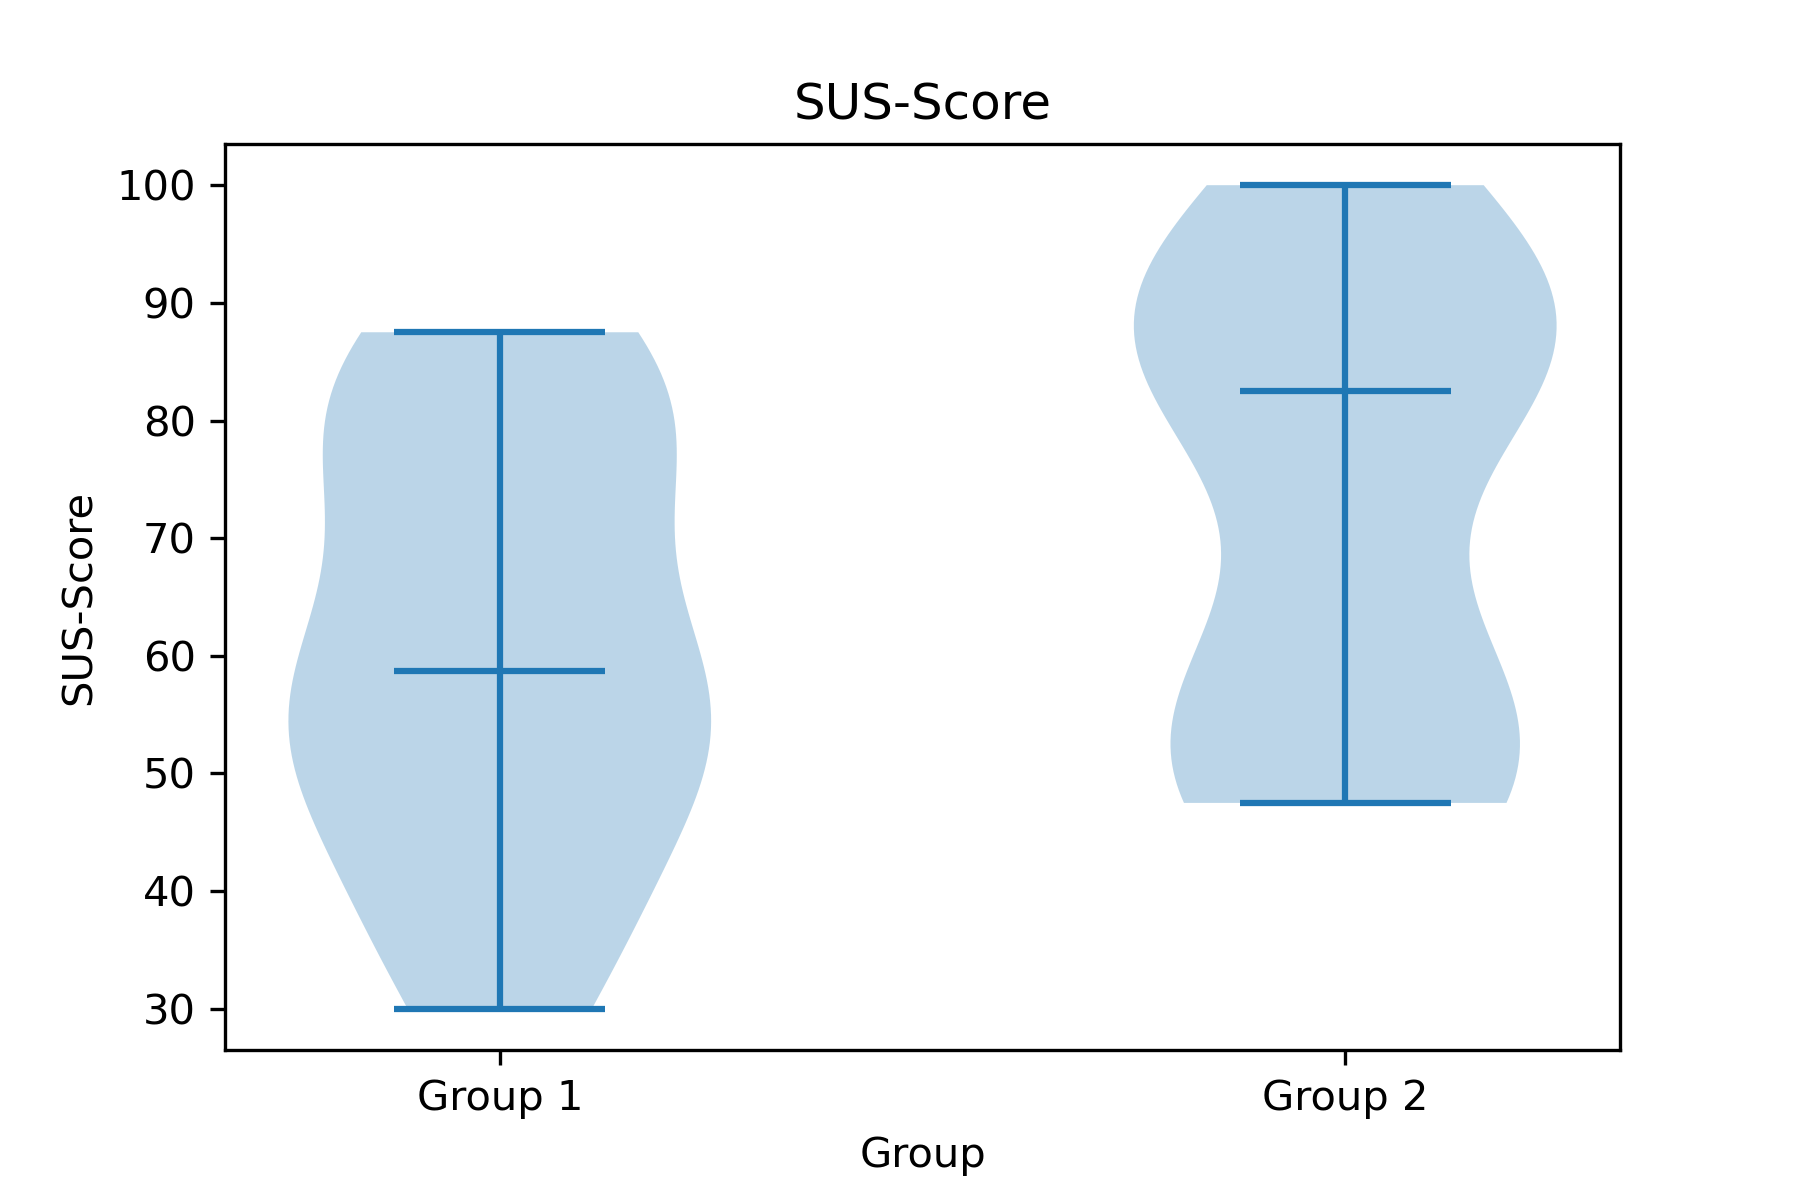
\includegraphics[width=1\textwidth]{Evaluation/img/SUS-Score_group_violin.png}
  \caption{The SUS-Scores of the two \gls{see} versions by group}\label{fig:sus-group-vio}
\end{figure}

Finally, comparing the \gls{sus}-Scores (figure \ref{fig:sus-vio}) of the two different versions shows that the null hypothesis $H_{e0}$ can be rejected since the \gls{utest} resulted in $U = 219.5; p \approx 0.035$.
The desktop version had an average \gls{sus}-Score of $\approx 73.06$ and a median of 78.75, while the mobile version had an average \gls{sus}-Score of $\approx 60.56$ and a median of 52.5. 
After seeing the results it can be assumed that the \gls{usability} of the desktop version is significantly higher than the \gls{usability} of the mobile version.
\begin{figure}[htb]
  \centering
  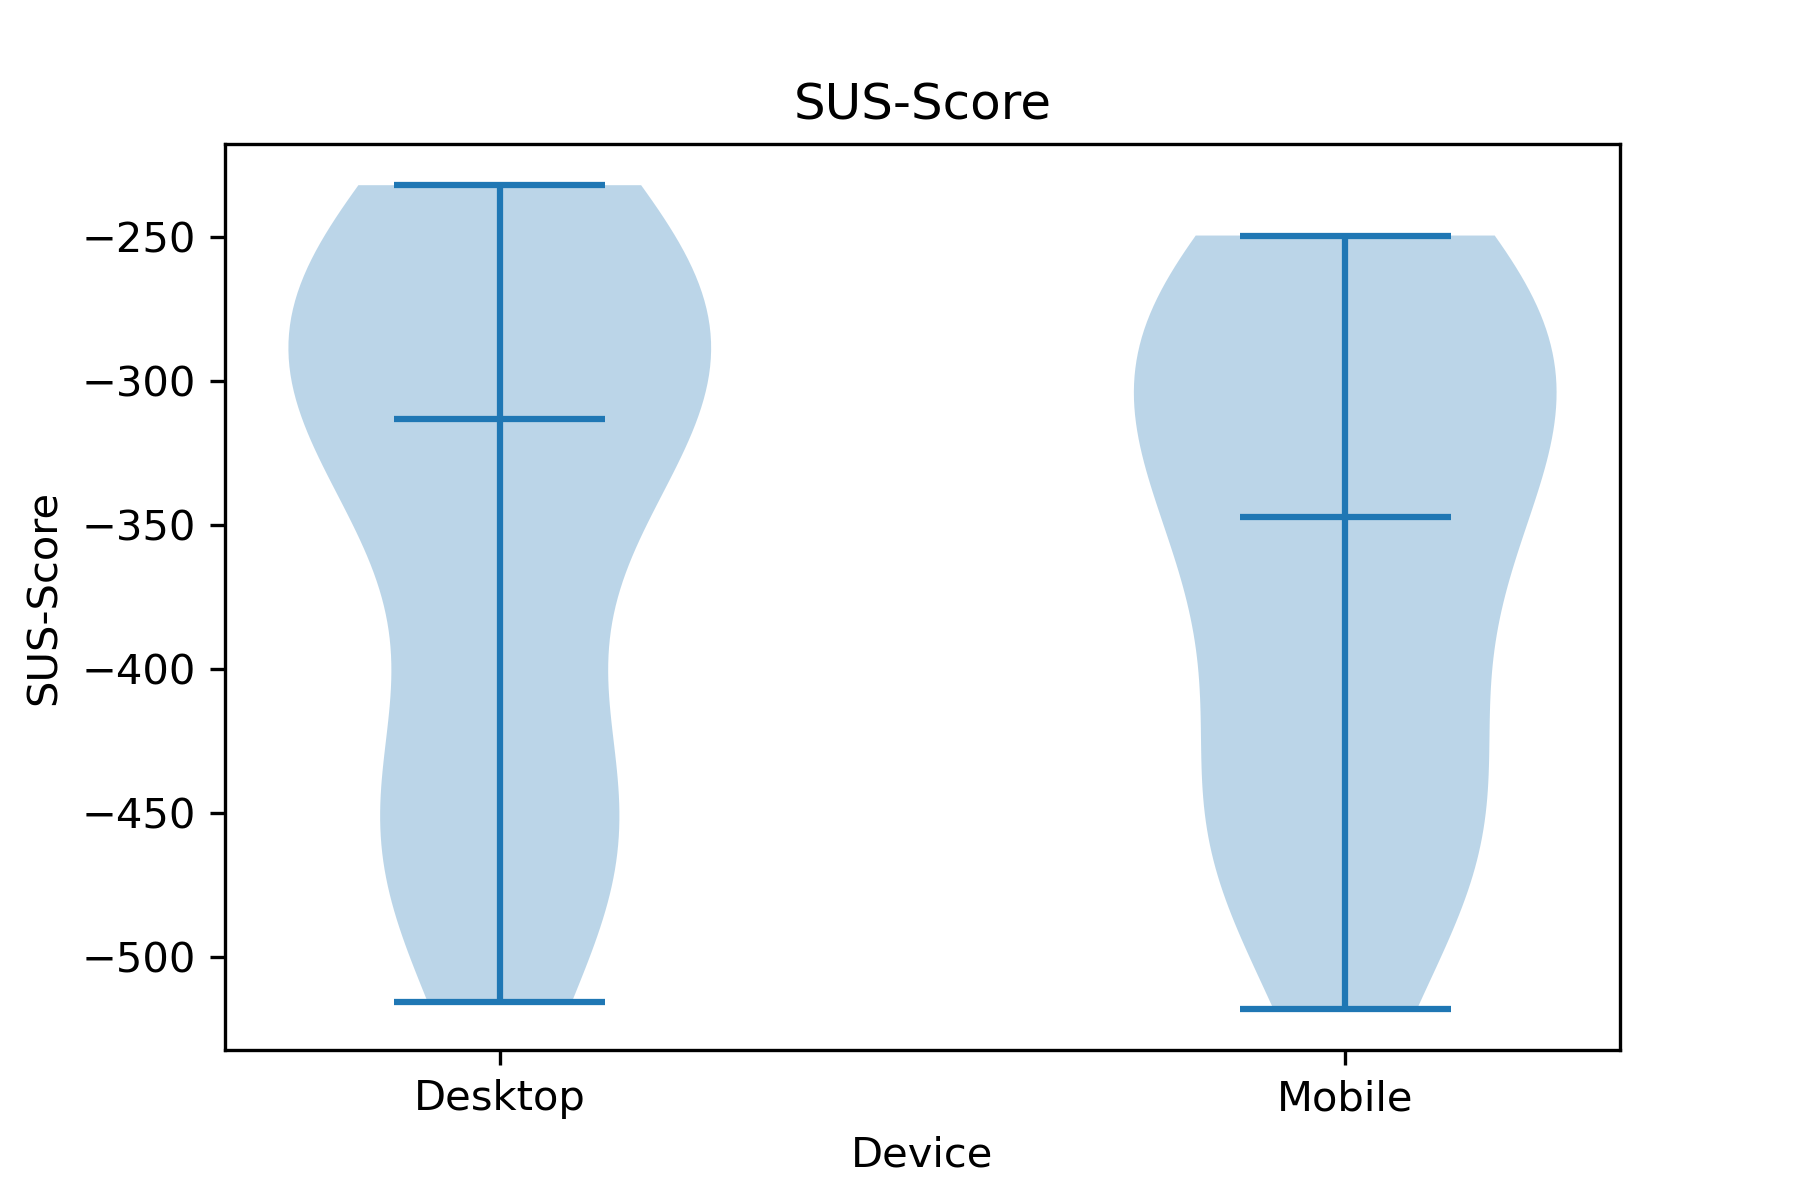
\includegraphics[width=1\textwidth]{Evaluation/img/SUS-Score_violin.png}
  \caption{The SUS-Scores of the two \gls{see} versions by device}\label{fig:sus-vio}
\end{figure}

\subsubsection{Impact of experience}
\label{sec:experinece}
As already described in section \ref{aim} the subjects will be grouped by their level of experience and their results analyzed.
Since only one subjects had no experience with first person video games but is still experienced with \gls{see} the subjects can be divided into three groups: 
\begin{itemize}
  \item \gls{see}-developer
  \item Non-\gls{see}-developer with software development experience
  \item Non-\gls{see}-developer without software development experience
\end{itemize}
In addition to that there will also be a look at the impact the highest achieved degree of the subjects has.
In order to measure the impact the \gls{tau} will be used.
Another option to calculate the correlation would have been Pearson’s correlation coefficient, which has been more popular, but its distribution has slightly worse statistical properties (\cite{hauke2011comparison}).
In addition to that \cite{khamis2008measures} also suggest the use of the \gls{tau}, if there is a small ordinal scale of less than five or six levels, which is the case for our results.

\paragraph{Experience with \gls{see}}\mbox{}\\
Table \ref{table:see-tau} contains the correlation between the experience with \gls{see} of the subjects and the dependent variable of the certain version of \gls{see}.
The significance level will be again $\alpha = 0.05$.
The only significant correlation was found for the \gls{sus}-Score with $\tau \approx 0.47$ and $p \approx 0.02$. 
That means that there is a weak positive correlation between the experience with \gls{see} and the \gls{sus}-Score.
This could be because subjects that worked with \gls{see} might be happy to see their work on a different device.

\begin{table}[]
  \resizebox{\textwidth}{!}{%
  \begin{tabular}{lllll}
  \hline
                    & \multicolumn{2}{l}{\textbf{SEE-Desktop}} & \multicolumn{2}{l}{\textbf{SEE-Mobile}} \\ \hline
  Performance       &  $\tau \approx -0.32;$ & $p \approx 0.12$   & $\tau \approx -0.37 ; $ & $p \approx 0.07 $ \\
  ASQ - Complexity  &  $\tau \approx 0.29;$  & $ p \approx 0.18$  & $\tau \approx 0.30;$    & $ p \approx 0.15 $ \\
  ASQ - Effort      &  $\tau \approx 0.19;$  & $ p \approx 0.37$  & $\tau \approx 0.16;$    & $ p \approx 0.46$ \\
  ASQ - Information &  $\tau \approx 0.04;$  & $ p \approx 0.87$  & $\tau \approx -0.03 ;$  & $ p \approx 0.88 $ \\
  SUS               &  $\tau \approx 0.29;$  & $ p \approx 0.17$  & \cellcolor[HTML]{FFFC9E} $\tau \approx 0.47;$ & \cellcolor[HTML]{FFFC9E} $ p \approx 0.02 $ \\ \\ \hline
  \end{tabular}%
  }
  \caption{Correlation between experience with \gls{see} and the dependent variables calculated with the \gls{tau}}
  \label{table:see-tau}
  \end{table}

\paragraph{Experience with software development}\mbox{}\\
The correlations between the experience with software development and the corresponding dependent variable from one of the two versions are listed in table \ref{table:sd-tau}.
For this comparison only the subjects without experience with \gls{see} were looked at.
Not a single significant correlation has been found in that context, which means that there is no impact the dependent variables by having experience with software development.

\begin{table}[htb]
  \resizebox{\textwidth}{!}{%
  \begin{tabular}{lllll}
  \hline
                    & \multicolumn{2}{l}{\textbf{SEE-Desktop}} & \multicolumn{2}{l}{\textbf{SEE-Mobile}} \\ \hline
  Performance       &  $\tau \approx -0.14;$ & $p \approx 0.56$   & $\tau \approx -0.07 ; $ & $p \approx 0.77 $ \\
  ASQ - Complexity  &  $\tau \approx -0.08;$  & $ p \approx 0.76$  & $\tau \approx 0.06;$    & $ p \approx 0.82 $ \\
  ASQ - Effort      &  $\tau \approx -0.21;$  & $ p \approx 0.41$  & $\tau \approx -0.05;$    & $ p \approx 0.83$ \\
  ASQ - Information &  $\tau \approx -0.39;$  & $ p \approx 0.15$  & $\tau \approx 0.21 ;$  & $ p \approx 0.41 $ \\
  SUS               &  $\tau \approx -0.07;$  & $ p \approx 0.77$  & $\tau \approx 0.04;$    & $ p \approx 0.88 $ \\ \\ \hline
  \end{tabular}%
  }
  \caption{Correlation between experience with software development and the dependent variables calculated with the \gls{tau} without the subjects that had experience with\gls{see}}
  \label{table:sd-tau}
  \end{table}

\paragraph{Highest achieved degree}\mbox{}\\
The correlations between the highest achieved degree and the corresponding dependent variable from one of the two versions can be found in table \ref{table:degree-tau}.
Also in this context the were no correlation even close to significance. 
This concludes that there is also no correlation between the highest achieved degree and the dependent variable.

\begin{table}[htb]
  \resizebox{\textwidth}{!}{%
  \begin{tabular}{lllll}
  \hline
                    & \multicolumn{2}{l}{\textbf{SEE-Desktop}} & \multicolumn{2}{l}{\textbf{SEE-Mobile}} \\ \hline
  Performance       &  $\tau \approx 0.06;$ & $p \approx 0.77$   & $\tau \approx -0.36 ; $ & $p \approx 0.06 $ \\
  ASQ - Complexity  &  $\tau \approx 0.06;$  & $ p \approx 0.76$  & $\tau \approx 0.10;$    & $ p \approx 0.62 $ \\
  ASQ - Effort      &  $\tau \approx -0.11;$  & $ p \approx 0.59$  & $\tau \approx 0.19;$    & $ p \approx 0.32$ \\
  ASQ - Information &  $\tau \approx 0.16;$  & $ p \approx 0.44$  & $\tau \approx 0.28 ;$  & $ p \approx 0.17 $ \\
  SUS               &  $\tau \approx 0.02;$  & $ p \approx 0.90$  & $\tau \approx 0.14;$    & $ p \approx 0.46 $ \\ \\ \hline
  \end{tabular}%
  }
  \caption{Correlation between highest achieved degree and the dependent variables calculated with the \gls{tau}}
  \label{table:degree-tau}
  \end{table}


\paragraph{Android version and device}\mbox{}\\
The correlations between the \gls{android} version or device and the corresponding dependent variable from one of the two versions can be found in table \ref{table:android-tau}.
The devices were divided into the once reported with a bad performance and the devices with and a mention of a bad performance.
Unfortunately it is not safe to say if the division is correct because it is possible that subjects did not mention the bad performance on their device.
There is still a significant correlation between the \gls{ASQ} effort aspect and the \gls{android} device.
A higher performing device means a weakly higher ASQ rating in the effort aspect, which is a positive effect since a high \gls{ASQ} score represents a low effort.
It is also to mention that the correlation between the \gls{android} device and the \gls{ASQ} complexity aspect is right on the edge the significance level of $\alpha = 0.05$.
It is quite possible that on another day it would fall below, which would signify that the there is also a positive correlation between a better performing device and a higher \gls{ASQ} complexity score.


\begin{table}[htb]
  \resizebox{\textwidth}{!}{%
  \begin{tabular}{lllll}
  \hline
                    & \multicolumn{2}{l}{\textbf{Android Version}} & \multicolumn{2}{l}{\textbf{Android device}} \\ \hline
  Performance       &  $\tau \approx -0.23;$ & $p \approx 0.22$   & $\tau \approx -0.35 ; $ & $p \approx 0.09 $ \\
  ASQ - Complexity  &  $\tau \approx 0.13;$  & $ p > 0.05$        & $\tau \approx 0.40;$    & $ p > 0.05 $ \\
  ASQ - Effort      &  $\tau \approx -0.02;$ & $ p \approx 0.91$  &\cellcolor[HTML]{FFFC9E} $\tau \approx 0.44;$    &\cellcolor[HTML]{FFFC9E}  $ p \approx 0.04$ \\
  ASQ - Information &  $\tau \approx 0.13;$  & $ p \approx 0.50$  & $\tau \approx 0.33;$    & $ p \approx 0.11 $ \\
  SUS               &  $\tau \approx 0.07;$  & $ p \approx 0.72$  & $\tau \approx 0.31;$    & $ p \approx 0.14 $ \\ \\ \hline
  \end{tabular}%
  }
  \caption{Correlation between the Android version or device and the dependent variables calculated with the \gls{tau}}
  \label{table:android-tau}
  \end{table}

\subsubsection{Comments of the subjects}
Last but not least the subjects were asked if they had suggestions for improvements or additional features.
The original answers can be found in \hyperref[group1]{See Desktop - See Mobile.csv } and \hyperref[group2]{See Mobile - See Desktop.csv}.
All the result have been grouped, commented and listed below: 

\paragraph{Desktop version}
\begin{itemize}
  \item Information on key assignments \textbf{x3}
  \begin{itemize}
    \item Since this was mentioned multiple times it might be considered to add some kind of information on the \glspl{shortcut}. An option would be to implement a tutorial mode, which offers this kind of information but can later be turned off after the user memorized the \glspl{shortcut}.
  \end{itemize}
  \item Better contrast or font for nodes and planes \textbf{x5}
  \begin{itemize}
    \item This was mentioned the most for the desktop version. This problem is already known and solutions are in progress. 
  \end{itemize}
  \item Easier switch between interaction modes
  \begin{itemize}
    \item This is already implemented with the key 1-9 but was not mentioned in the tutorial video since it is not beginner-friendly and the subjects should not be confronted with too much information to memorize.
  \end{itemize}
  \item Hard to use without a mouse
  \begin{itemize}
    \item This is not optimized yet. Maybe it is worth considering an option to work only with a touchpad or just to clarify that a mouse is needed for an optimal use of \gls{see} desktop.
  \end{itemize}
  \item Visible UI elements, key combinations are hard to remember
  \begin{itemize}
    \item Eventually pressing \glspl{shortcut} like \enquote{alt} in the rotate mode could be indicated as well. 
  \end{itemize}
\end{itemize} 
\paragraph{Mobile version}
\begin{itemize}
  \item Different colors for menu buttons and sub menu buttons 
  \begin{itemize}
    \item The UI design seemed to be confusing for some subjects. 
    Maybe a division of the main button that also reopens the menu again and the additional buttons should be considered. 
    Different colors could be an option or different icons for the main buttons that also indicate the menu can be opened. 
  \end{itemize}
  \item Less battery usage
  \begin{itemize}
    \item This is probably due to the high need of computing power of \gls{see}. \gls{see} is in ongoing development and on optimizing the efficiency is always a topic. 
  \end{itemize}
  \item Better icons \textbf{x2}
  \begin{itemize}
    \item One subject mentioned that the minus icon for adding an edge is confusing since a minus rather indicates to delete something. 
    Most of the icons are the same in both versions, but the desktop version also contains a button title. 
    Designing a set of homogeneous and innovative icons might be worth considering.
  \end{itemize}
  \item Deselect button should always be available 
  \begin{itemize}
    \item This can easily be fixed by moving the button into the \enquote{quickmenu}, which is available from every interaction mode.
  \end{itemize}
  \item The camera notches of some devices overlap some buttons \textbf{x2}
  \begin{itemize}
    \item A general approach for this would be to not allow screen space with a notch on it. 
    This would sacrifice screen space but provide consistency over different devices. 
    Having a design for every possible device seems to be too much effort.
  \end{itemize}
  \item Joysticks to far in the corner
  \begin{itemize}
    \item Since this did not apply for the testing device, there might need to be found a more dynamic approach which considers the actual screen size and adapts the UI size to it. 
  \end{itemize}
  \item Joystick handling to sensitive 
  \begin{itemize}
    \item This seemed to be an issue for more than one subjects even if only one mentioned it. The sensitivity should probably be reduced. That way the user can work more precisely.
  \end{itemize}
  \item Zooming inverted \textbf{x9}
  \begin{itemize}
    \item Since this was explicitly mentioned by half the subjects, this should definitely be changed. 
  \end{itemize}
  \item Better performance on older devices
  \begin{itemize}
    \item This is probably hard implement. Maybe optimizing features of \gls{see} that require heavy computing will help in the future.
  \end{itemize}
  \item App layout should be turned by 180° \textbf{x2}
  \begin{itemize}
    \item This can be adjusted in the Unity editor and is an easy fix. 
  \end{itemize}
  \item Add a search function
  \begin{itemize}
    \item This could be considered for the future since the desktop version already has a search option.
  \end{itemize}
  \item Sometimes planes were deleted after I changed the mode from delete
  \begin{itemize}
    \item The menu and joysticks need to be safe to touch. Right now objects below buttons or joysticks get selected.
  \end{itemize}
\end{itemize} 

\subsection{Threads to validity}
\label{sec:validity}
This chapter will be closed with a discussion on the threads of validity to the executed study.
For this purpose, there will be a distinction into \textit{internal validity} and \textit{external validity} as by \cite{campbell2015experimental}

\subsubsection{Internal Validity}
The internal validity is about the correlation between the independent variable, which is the version of \gls{see} in this case, and the dependent variable, which is \textit{performance}, \textit{\gls{ASQ}-Score} and \textit{\gls{sus}-Score}.
Some of \cite{campbell2015experimental} factors will be discussed in the following.

\paragraph{History}\mbox{}\\
The subjects did the study asynchronously and there is no significant difference between the time it took place for the two groups as seen in figure \ref{fig:date_violin}.
The study took place within five days. 
It is very unlikely that one of the subjects could have gotten an advantage by for example trying out \gls{see} because every subject got the applications just shortly before their appointment.

\begin{figure}[htb]
  \centering
  \includegraphics*[width=1\textwidth]{Evaluation/img/_violin_time.png}
  \caption{The time the subjects started the experiment}
  \label{fig:date_violin}
\end{figure}

\paragraph{Testing}\mbox{}\\
There could be a learning effect since the tasks were comparable to each other. 
To prevent a learning effect the subjects got a training before the time was measured in the actual tasks.
The training contained all necessary interactions to solve the tasks and since the interactions are executed in different ways in the two versions the learning effect should not be to high if even exciting.

\paragraph{Instrumentation}\mbox{}\\
Unfortunately the performance on the subjects \gls{android} devices fluctuated quite much and there was also a significant correlation between the performance of the \gls{android} device and the \gls{ASQ} aspect of \textit{effort} as described in section \ref{sec:experinece}.
Furthermore, it can also not be ruled out that the performance of the desktop device had an inpact on the results even if no subjects mentioned any troubles.
\paragraph{Biases}\mbox{}\\
Many of the subjects know me personally and most of them also knew that I did the mobile implementation of \gls{see}. 
It is therefore possible that they gave a higher rating. 
There was also found a correlation between subjects experienced with \gls{see} and the \gls{sus} score in section \ref{sec:experinece}, which could be caused because \gls{see} developers are most likely emotional involved in the project.
Since there is no significant difference of the amount of \gls{see} experienced subjects this should not have impact on the study results but could still be a thread to validity.
\paragraph{Selection}\mbox{}\\
The selection of the subjects was random, however it is still possible that the groups would have been formed uneven.
In section \ref{sec:demo} no significant difference between the two groups was found.
Still in section \ref{sec:usability} significant differences between the \gls{ASQ} ratings the two groups gave were found.
Therefore, this thread to validity can not be excluded. 
\paragraph{Other Threads}\mbox{}\\
The \glspl{city} of the two task blocks were not the same. 
This is to reduce the learning effect, but it is possible that they differed in complexity and had impact on the difficulty of the tasks.
However, the \glspl{city} are at least similar as discussed in \ref{pilot}
\subsubsection{External Validity}
External validity looks at the generalizability of a study.
Are the findings appliable in general or just for this specific case?
However, the question of generalizability can never be fully answered and there can only be approximations. 
Threads to the external validity could be:

\paragraph{Nonrepresentative Sample}\mbox{}\\
Unfortunately the subjects do not fully represent the population of the software development industry as all the subjects are male and 16 of 18 subjects are in the age of 12-30 years.
In addition to that most of the subjects are not even software developers.

\paragraph{Reactive effects of experimental arrangement}\mbox{}\\
Since the study was supervised the subjects might felt observed, which could have an impact on there performance.
The environmental conditions of the real use of \gls{see} cannot be reproduced in an experimental arrangement.
The external validity is therefore in doubt.